\documentclass[utf8, 14pt]{roc-class}
\onehalfspacing
\setcounter{tocdepth}{4}

\usepackage{titletoc}
%\titlecontents{subsection}
%[1.5em] %
%{\smallskip}
%{\thecontentslabel\hspace{1.02em}}%\thecontentslabel
%{\hspace*{2.32em}}
%{\,\,\titlerule*[0.77pc]{.}\contentspage}

\begin{document}
    
    % Первая страница
    \fancypagestyle{firststyle}
    {
        \fancyhead{}
        \fancyfoot{}
        \fancyhead{}
    }
    
    \thispagestyle{firststyle}
    
    \vspace*{\fill}
    \begin{center}
        \Huge
        
        Rise of Cultures
        
        \bigskip
        
        УСТАВ АЛЬЯНСА
        
        BlackDragon
    \end{center}
    \vspace*{\fill}
    \begin{center}
        decodermail@gmail.com
    \end{center}

    \newpage
    
    {
        \hypersetup{linkcolor=black}
        \tableofcontents
    }
    
    \newpage
    
    Мы, члены Альянса BlackDragon сплочённо действуем ради общей цели сохранять свои позиции не менее 50"~го места среди прочих альянсов нашего сервера.
    Мы строго соблюдаем описанные ниже правила и советы для достижения нашей Цели!
    
    \bigskip
    
    Данный документ будет дополняться и редактироваться со временем.
    Свежую версию всегда можно найти на \underline{\href{https://github.com/decodergit/RoC-BlackDragon}{GitHub}}.
    
    \section{Чудеса Света}

\subsection{Правила инвестирования}

В нашем Альянсе принята особая стратегия вложений в Чудеса Света.
Главное правило -- мы вкладываем только в Чудеса членов нашего Альянса.
Каждый желающий получить призовое место должен вложить
$$\frac{N}{2^i}$$
колб, где $N$ -- общее число колб, которые необходимо вложить для улучшения чуда, а $i \geqslant 1$ -- место, которое вкладчик желает занять.

То есть, претендент на первое место обязан вложить ровно половину колб. 
На второе -- ровно четверть. 
На третье -- восьмую часть... 

Хозяин Чуда обязан закрыть остаток, если в процессе этого уже не сделали вражеские агенты. 

Чтобы убрать внутреннюю конкуренцию предлагаю поступать следующим образом. 

Первое место получает тот, кто раньше других успел вложить четверть от общего количества колб. 
Второе место -- раньше всех вложивший восьмую часть колб...

Основное -- это обязанность вкладывать заданное число колб даже в случае повышенной активности вражеских агентов. Мы просто не обращаем на них внимания. Такие вложения не дадут им шансов.

Поясню на простом примере. Предположим есть Чудо на 200 колб и врагов пока нет. Первый вкладывает 100, второй 50, третий 25. Три призовые места заняты. Их не сместить. Хозяин может докидывать оставшиеся 25 колб. Если враг уже вложил не менее 25 колб, хозяин может ничего не добавлять.

Рассмотрим на примере, как выбрать чудо для вложения: у Вас нет технологий для вложения колб.
Ни в коем случае не вкладывайте в своё Чудо.
Это сделают другие, чтобы в альянс поступали призовые колбы и чертежи.
Пробегитесь по списку альянса и найдите Чудо для вложения.
Вот приоритезированный список для вложения (сначала следует выбирать категорию, затем подкатегорию затем категорию третьего уровня в порядке убывания приоритета):

\begin{itemize}
    \item  Уже вкладываете в какое-то чудо:
    \begin{enumerate}
        \item вкладывайте в него.
    \end{enumerate}
    
    \item список вложений пуст:
    \begin{enumerate}
        \item закончились чертежи какого-то Чуда (начинать выбор с чуда с минимальным уровнем):
        \begin{enumerate}
            \item если доступно, вкладывайте в Чудо с минимальным уровнем члена данной TELEGRAM-группы;
            \item если доступно, вкладывайте в Чудо с минимальным уровнем АКТИВНОГО члена альянса;
            \item если доступно, вкладывайте в Чудо с минимальным уровнем члена альянса, который с нами НЕ МЕНЕЕ 3 НЕДЕЛЬ;
            \item сделайте вложение в любое чудо членов альянса (с~приоритетами~а-в), где можно занять призовое место;
            \item сделайте вложение в любое чудо членов альянса (с~приоритетами~а-в).
        \end{enumerate}
        \item чертежей для своих Чудес достаточно:
        \begin{enumerate}
            \item если доступно, вкладывайте в Чудо с минимальным уровнем члена данной TELEGRAM-группы;
            \item если доступно, вкладывайте в Чудо с минимальным уровнем АКТИВНОГО члена альянса;
            \item если доступно, вкладывайте в Чудо с минимальным уровнем члена альянса, который с нами НЕ МЕНЕЕ 3 НЕДЕЛЬ;
            \item сделайте вложение в любое чудо членов альянса (с~приоритетами~а-в), где можно занять призовое место;
            \item сделайте вложение в любое чудо членов альянса (с~приоритетами~а-в).
        \end{enumerate}
    \end{enumerate}
\end{itemize}

При прочих равных для прокачки имеет смысл выбирать чудеса в следующем порядке:

\begin{enumerate}
    \item Статуя Зевса;
    \item Стоунхендж;
    \item Висячие Сады
\end{enumerate}

Такой порядок обусловлен следующим:

\begin{enumerate}
    \item Понятно, что перманентное усиление армии в приоритете;
    \item Стоунхендж с 10-го уровня дают ещё одну колбу;
    \item Висячие сады с 15-го уровня дают ещё одного рабочего.
\end{enumerate}

До рабочего просто намного дольше качать.


\subsection{Призовые места}

Здесь приведены переработанные таблицы со
\underline{\href{https://rise-of-cultures.fandom.com/wiki/World\_Wonders}{страницы}}
фанатской вики.
Там они не очень удобны и разбросаны по разным местам.
Собирают информацию они постепенно. Поэтому таблицы могут быть не полными.

\subsubsection{Стоунхендж}

\begin{longtable}[c]{|c|c|c|c|c|c|c|c|}
    \hline
    \multirow{ 2}{*}{\small Уровень} &
    \multicolumn{2}{|c|}{\small Нужно} &
    \multirow{ 2}{*}{\small Место} & 
    \multirow{ 2}{*}{\small Инвестиция} & 
    \multicolumn{3}{|c|}{\small Приз} \\\cline{2-3}\cline{6-8}
    &
    {\small Колб} & 
    {\small Чертежей} & 
    & &
    {\small Колб} & 
    {\small Чертежей} & 
    {\small Профит}
    \\\hline\endhead
    \multirow{1}{*}{1} & \multirow{1}{*}{2} & \multirow{1}{*}{5} & 1 & 1 & 3 & 1 & 3.00 \\\hline
    \multirow{2}{*}{2} & \multirow{2}{*}{10} & \multirow{2}{*}{5} & 1 & 5 & 5 & 2 & 1.00 \\\cline{4-8}
    & & & 3 & 3 & 3 & 1 & 1.00 \\\hline
    \multirow{2}{*}{3} & \multirow{2}{*}{15} & \multirow{2}{*}{5} & 1 & 8 & 5 & 3 & 0.62 \\\cline{4-8}
    & & & 3 & 4 & 3 & 1 & 0.75 \\\hline
    \multirow{3}{*}{4} & \multirow{3}{*}{40} & \multirow{3}{*}{6} & 1 & 20 & 10 & 3 & 0.50 \\\cline{4-8}
    & & & 3 & 10 & 5 & 2 & 0.50 \\\cline{4-8}
    & & & 4 & 5 & 5 & 1 & 1.00 \\\hline
    \multirow{3}{*}{5} & \multirow{3}{*}{120} & \multirow{3}{*}{6} & 1 & 60 & 20 & 3 & 0.33 \\\cline{4-8}
    & & & 3 & 30 & 10 & 2 & 0.33 \\\cline{4-8}
    & & & 4 & 15 & 5 & 1 & 0.33 \\\hline
    \multirow{4}{*}{6} & \multirow{4}{*}{200} & \multirow{4}{*}{7} & 1 & 100 & 25 & 3 & 0.25 \\\cline{4-8}
    & & & 3 & 50 & 15 & 2 & 0.30 \\\cline{4-8}
    & & & 4 & 25 & 10 & 1 & 0.40 \\\cline{4-8}
    & & & 5 & 13 & 5 & 0 & 0.38 \\\hline
    \multirow{4}{*}{7} & \multirow{4}{*}{260} & \multirow{4}{*}{7} & 1 & 130 & 35 & 3 & 0.27 \\\cline{4-8}
    & & & 3 & 65 & 20 & 2 & 0.31 \\\cline{4-8}
    & & & 4 & 33 & 10 & 1 & 0.30 \\\cline{4-8}
    & & & 5 & 17 & 5 & 0 & 0.29 \\\hline
    \multirow{4}{*}{8} & \multirow{4}{*}{330} & \multirow{4}{*}{8} & 1 & 165 & 40 & 3 & 0.24 \\\cline{4-8}
    & & & 3 & 83 & 25 & 2 & 0.30 \\\cline{4-8}
    & & & 4 & 42 & 10 & 1 & 0.24 \\\cline{4-8}
    & & & 5 & 21 & 5 & 0 & 0.24 \\\hline
    \multirow{4}{*}{9} & \multirow{4}{*}{410} & \multirow{4}{*}{8} & 1 & 205 & 50 & 3 & 0.24 \\\cline{4-8}
    & & & 3 & 103 & 30 & 2 & 0.29 \\\cline{4-8}
    & & & 4 & 52 & 15 & 1 & 0.29 \\\cline{4-8}
    & & & 5 & 26 & 5 & 0 & 0.19 \\\hline
    \multirow{4}{*}{10} & \multirow{4}{*}{500} & \multirow{4}{*}{9} & 1 & 250 & 55 & 3 & 0.22 \\\cline{4-8}
    & & & 3 & 125 & 35 & 2 & 0.28 \\\cline{4-8}
    & & & 4 & 63 & 15 & 1 & 0.24 \\\cline{4-8}
    & & & 5 & 32 & 5 & 0 & 0.16 \\\hline
    \multirow{4}{*}{11} & \multirow{4}{*}{560} & \multirow{4}{*}{9} & 1 & 280 & 60 & 3 & 0.21 \\\cline{4-8}
    & & & 3 & 140 & 35 & 2 & 0.25 \\\cline{4-8}
    & & & 4 & 70 & 15 & 1 & 0.21 \\\cline{4-8}
    & & & 5 & 35 & 5 & 0 & 0.14 \\\hline
    \multirow{1}{*}{12} & \multirow{1}{*}{580} & \multirow{1}{*}{10} & & & & & \\\hline
    \multirow{1}{*}{13} & \multirow{1}{*}{610} & \multirow{1}{*}{10} & & & & & \\\hline
    \multirow{4}{*}{14} & \multirow{4}{*}{640} & \multirow{4}{*}{11} & 1 & 320 & 65 & 3 & 0.20 \\\cline{4-8}
    & & & 3 & 160 & 40 & 2 & 0.25 \\\cline{4-8}
    & & & 4 & 80 & 20 & 1 & 0.25 \\\cline{4-8}
    & & & 5 & 40 & 5 & 0 & 0.12 \\\hline
    \multirow{1}{*}{15} & \multirow{1}{*}{660} & \multirow{1}{*}{11} & & & & & \\\hline
    \multirow{1}{*}{16} & \multirow{1}{*}{690} & \multirow{1}{*}{12} & & & & & \\\hline
    \multirow{1}{*}{17} & \multirow{1}{*}{720} & \multirow{1}{*}{12} & & & & & \\\hline
\end{longtable}


\subsubsection{Висячие Сады}

\begin{longtable}[c]{|c|c|c|c|c|c|c|c|}
    \hline
    \multirow{ 2}{*}{\small Уровень} &
    \multicolumn{2}{|c|}{\small Нужно} &
    \multirow{ 2}{*}{\small Место} & 
    \multirow{ 2}{*}{\small Инвестиция} & 
    \multicolumn{3}{|c|}{\small Приз} \\\cline{2-3}\cline{6-8}
    &
    {\small Колб} & 
    {\small Чертежей} & 
    & &
    {\small Колб} & 
    {\small Чертежей} & 
    {\small Профит}
    \\\hline\endhead
    \multirow{1}{*}{1} & \multirow{1}{*}{5} & \multirow{1}{*}{5} & 1 & 3 & 5 & 1 & 1.67 \\\hline
    \multirow{2}{*}{2} & \multirow{2}{*}{10} & \multirow{2}{*}{5} & 1 & 5 & 5 & 2 & 1.00 \\\cline{4-8}
    & & & 3 & 3 & 3 & 1 & 1.00 \\\hline
    \multirow{3}{*}{3} & \multirow{3}{*}{25} & \multirow{3}{*}{5} & 1 & 13 & 5 & 3 & 0.38 \\\cline{4-8}
    & & & 3 & 7 & 5 & 2 & 0.71 \\\cline{4-8}
    & & & 4 & 4 & 3 & 1 & 0.75 \\\hline
    \multirow{3}{*}{4} & \multirow{3}{*}{60} & \multirow{3}{*}{6} & 1 & 30 & 15 & 3 & 0.50 \\\cline{4-8}
    & & & 3 & 15 & 10 & 2 & 0.67 \\\cline{4-8}
    & & & 4 & 8 & 5 & 1 & 0.62 \\\hline
    \multirow{3}{*}{5} & \multirow{3}{*}{140} & \multirow{3}{*}{6} & 1 & 70 & 20 & 3 & 0.29 \\\cline{4-8}
    & & & 3 & 35 & 10 & 2 & 0.29 \\\cline{4-8}
    & & & 4 & 18 & 5 & 1 & 0.28 \\\hline
    \multirow{4}{*}{6} & \multirow{4}{*}{200} & \multirow{4}{*}{7} & 1 & 100 & 25 & 3 & 0.25 \\\cline{4-8}
    & & & 3 & 50 & 15 & 2 & 0.30 \\\cline{4-8}
    & & & 4 & 25 & 10 & 1 & 0.40 \\\cline{4-8}
    & & & 5 & 13 & 5 & 0 & 0.38 \\\hline
    \multirow{4}{*}{7} & \multirow{4}{*}{260} & \multirow{4}{*}{7} & 1 & 130 & 35 & 3 & 0.27 \\\cline{4-8}
    & & & 3 & 65 & 20 & 2 & 0.31 \\\cline{4-8}
    & & & 4 & 33 & 10 & 1 & 0.30 \\\cline{4-8}
    & & & 5 & 17 & 5 & 0 & 0.29 \\\hline
    \multirow{4}{*}{8} & \multirow{4}{*}{330} & \multirow{4}{*}{8} & 1 & 165 & 40 & 3 & 0.24 \\\cline{4-8}
    & & & 3 & 83 & 25 & 2 & 0.30 \\\cline{4-8}
    & & & 4 & 42 & 10 & 1 & 0.24 \\\cline{4-8}
    & & & 5 & 21 & 5 & 0 & 0.24 \\\hline
    \multirow{2}{*}{9} & \multirow{2}{*}{410} & \multirow{2}{*}{8} & 1 & 205 & 50 & 3 & 0.24 \\\cline{4-8}
    & & & 3 & 103 & 30 & 2 & 0.29 \\\hline
    \multirow{1}{*}{10} & \multirow{1}{*}{500} & \multirow{1}{*}{9} & 1 & 250 & 55 & 3 & 0.22 \\\hline
    \multirow{1}{*}{11} & \multirow{1}{*}{560} & \multirow{1}{*}{9} & & & & & \\\hline
    \multirow{1}{*}{12} & \multirow{1}{*}{580} & \multirow{1}{*}{10} & & & & & \\\hline
    \multirow{1}{*}{13} & \multirow{1}{*}{610} & \multirow{1}{*}{10} & & & & & \\\hline
    \multirow{1}{*}{14} & \multirow{1}{*}{640} & \multirow{1}{*}{11} & & & & & \\\hline
    \multirow{1}{*}{15} & \multirow{1}{*}{660} & \multirow{1}{*}{11} & & & & & \\\hline
    \multirow{1}{*}{16} & \multirow{1}{*}{690} & \multirow{1}{*}{12} & & & & & \\\hline
    \multirow{1}{*}{17} & \multirow{1}{*}{720} & \multirow{1}{*}{12} & & & & & \\\hline
    \multirow{1}{*}{18} & \multirow{1}{*}{740} & \multirow{1}{*}{13} & & & & & \\\hline
    \multirow{1}{*}{19} & \multirow{1}{*}{770} & \multirow{1}{*}{13} & & & & & \\\hline
    \multirow{1}{*}{20} & \multirow{1}{*}{800} & \multirow{1}{*}{14} & & & & & \\\hline
    \multirow{1}{*}{21} & \multirow{1}{*}{830} & \multirow{1}{*}{14} & & & & & \\\hline
    \multirow{1}{*}{22} & \multirow{1}{*}{860} & \multirow{1}{*}{15} & & & & & \\\hline
    \multirow{1}{*}{23} & \multirow{1}{*}{890} & \multirow{1}{*}{15} & & & & & \\\hline
    \multirow{1}{*}{24} & \multirow{1}{*}{920} & \multirow{1}{*}{16} & & & & & \\\hline
    \multirow{1}{*}{25} & \multirow{1}{*}{950} & \multirow{1}{*}{16} & & & & & \\\hline
    \multirow{1}{*}{26} & \multirow{1}{*}{980} & \multirow{1}{*}{17} & & & & & \\\hline
\end{longtable}


\subsubsection{Статуя Зевса}

\begin{longtable}[c]{|c|c|c|c|c|c|c|c|}
    \hline
    \multirow{ 2}{*}{\small Уровень} &
    \multicolumn{2}{|c|}{\small Нужно} &
    \multirow{ 2}{*}{\small Место} & 
    \multirow{ 2}{*}{\small Инвестиция} & 
    \multicolumn{3}{|c|}{\small Приз} \\\cline{2-3}\cline{6-8}
    &
    {\small Колб} & 
    {\small Чертежей} & 
    & &
    {\small Колб} & 
    {\small Чертежей} & 
    {\small Профит}
    \\\hline\endhead
\end{longtable}


\subsubsection{Храм Артемиды}

\begin{longtable}[c]{|c|c|c|c|c|c|c|c|}
    \hline
    \multirow{ 2}{*}{\small Уровень} &
    \multicolumn{2}{|c|}{\small Нужно} &
    \multirow{ 2}{*}{\small Место} & 
    \multirow{ 2}{*}{\small Инвестиция} & 
    \multicolumn{3}{|c|}{\small Приз} \\\cline{2-3}\cline{6-8}
    &
    {\small Колб} & 
    {\small Чертежей} & 
    & &
    {\small Колб} & 
    {\small Чертежей} & 
    {\small Профит}
    \\\hline\endhead
    \multirow{1}{*}{1} & \multirow{1}{*}{20} & \multirow{1}{*}{20} & 1 & 10 & 5 & 1 & 0.50 \\\hline
    \multirow{2}{*}{2} & \multirow{2}{*}{30} & \multirow{2}{*}{5} & 1 & 15 & 10 & 2 & 0.67 \\\cline{4-8}
    & & & 3 & 8 & 5 & 1 & 0.62 \\\hline
\end{longtable}


\subsubsection{Колизей}

\begin{longtable}[c]{|c|c|c|c|c|c|c|c|}
    \hline
    \multirow{ 2}{*}{\small Уровень} &
    \multicolumn{2}{|c|}{\small Нужно} &
    \multirow{ 2}{*}{\small Место} & 
    \multirow{ 2}{*}{\small Инвестиция} & 
    \multicolumn{3}{|c|}{\small Приз} \\\cline{2-3}\cline{6-8}
    &
    {\small Колб} & 
    {\small Чертежей} & 
    & &
    {\small Колб} & 
    {\small Чертежей} & 
    {\small Профит}
    \\\hline\endhead
    \multirow{1}{*}{1} & \multirow{1}{*}{35} & \multirow{1}{*}{20} & & & & & \\\hline
    \multirow{1}{*}{2} & \multirow{1}{*}{55} & \multirow{1}{*}{5} & & & & & \\\hline
    \multirow{1}{*}{3} & \multirow{1}{*}{80} & \multirow{1}{*}{5} & & & & & \\\hline
    \multirow{1}{*}{4} & \multirow{1}{*}{115} & \multirow{1}{*}{6} & & & & & \\\hline
    \multirow{1}{*}{5} & \multirow{1}{*}{160} & \multirow{1}{*}{6} & & & & & \\\hline
    \multirow{1}{*}{6} & \multirow{1}{*}{215} & \multirow{1}{*}{7} & & & & & \\\hline
    \multirow{1}{*}{7} & \multirow{1}{*}{280} & \multirow{1}{*}{7} & & & & & \\\hline
    \multirow{1}{*}{8} & \multirow{1}{*}{355} & \multirow{1}{*}{8} & & & & & \\\hline
    \multirow{1}{*}{9} & \multirow{1}{*}{440} & \multirow{1}{*}{8} & & & & & \\\hline
    \multirow{1}{*}{10} & \multirow{1}{*}{540} & \multirow{1}{*}{9} & & & & & \\\hline
    \multirow{1}{*}{11} & \multirow{1}{*}{600} & \multirow{1}{*}{9} & & & & & \\\hline
    \multirow{1}{*}{12} & \multirow{1}{*}{630} & \multirow{1}{*}{10} & & & & & \\\hline
    \multirow{1}{*}{13} & \multirow{1}{*}{650} & \multirow{1}{*}{10} & & & & & \\\hline
    \multirow{1}{*}{14} & \multirow{1}{*}{680} & \multirow{1}{*}{11} & & & & & \\\hline
\end{longtable}


\subsubsection{Софийский Собор}

\begin{longtable}[c]{|c|c|c|c|c|c|c|c|}
    \hline
    \multirow{ 2}{*}{\small Уровень} &
    \multicolumn{2}{|c|}{\small Нужно} &
    \multirow{ 2}{*}{\small Место} & 
    \multirow{ 2}{*}{\small Инвестиция} & 
    \multicolumn{3}{|c|}{\small Приз} \\\cline{2-3}\cline{6-8}
    &
    {\small Колб} & 
    {\small Чертежей} & 
    & &
    {\small Колб} & 
    {\small Чертежей} & 
    {\small Профит}
    \\\hline\endhead
\end{longtable}


\subsubsection{Ахенский Дворец}

\begin{longtable}[c]{|c|c|c|c|c|c|c|c|}
    \hline
    \multirow{ 2}{*}{\small Уровень} &
    \multicolumn{2}{|c|}{\small Нужно} &
    \multirow{ 2}{*}{\small Место} & 
    \multirow{ 2}{*}{\small Инвестиция} & 
    \multicolumn{3}{|c|}{\small Приз} \\\cline{2-3}\cline{6-8}
    &
    {\small Колб} & 
    {\small Чертежей} & 
    & &
    {\small Колб} & 
    {\small Чертежей} & 
    {\small Профит}
    \\\hline\endhead
    \multirow{1}{*}{1} & \multirow{1}{*}{75} & \multirow{1}{*}{20} & & & & & \\\hline
    \multirow{1}{*}{2} & \multirow{1}{*}{55} & \multirow{1}{*}{5} & & & & & \\\hline
    \multirow{1}{*}{3} & \multirow{1}{*}{80} & \multirow{1}{*}{5} & & & & & \\\hline
    \multirow{1}{*}{4} & \multirow{1}{*}{115} & \multirow{1}{*}{6} & & & & & \\\hline
    \multirow{1}{*}{5} & \multirow{1}{*}{160} & \multirow{1}{*}{6} & & & & & \\\hline
    \multirow{1}{*}{6} & \multirow{1}{*}{215} & \multirow{1}{*}{7} & & & & & \\\hline
\end{longtable}

    \section{Бой}

\subsection{Расстановка}

В любом бою старайтесь расставить войска максимально плотно, чтобы минимизировать число пустых клеток.

На переднем крае всегда должна быть пехота (обычная или тяжёлая).

Лучники вегда должны быть сзади.
Если у врага есть конница, лучников необходимо ставить либо за двумя слоями пехоты (в основном это касается компании -- в Сокровищах таких больших карт нет), либо за тяжёлой пехотой (но с соблюдением правила максимизации плотности расстановки).

Если у врага дальнобойные войска закрыты тяжёлой пехотой, конников нужно ставить сзади.
Особенно это касается боёв с двумя волнами.
Так вы сможете сэкономить коней на вторую волну.

И если на второй волне остались только лучники, ставьте их в дальнем углу.
За время, пока войска бегут друг к другу, у Вас почти успеет активироваться Командир (щит для лучников).

\subsection{Командиры}

Всех командиров, призывающих войска нужно сбрасывать непосредственно на головы врага.
Так они наносят дополнительный урон, но только если готовы принять выбранную Вами цель в качестве своей.

Не всегда стоит торопиться бросать командиров с войсками в бой.
Иногда бывает так, что у вас остаются лучники и какая-то горстка войск.
Лучше подождать пока враг уничтожит эти войска, и сразу следом кидать новые.
Так у лучников появляется больше времени на нанесение урона.

\textbf{Минос}

Теоретически Минос, будучи конницей, должен оставаться на заднем фланге врага и бить лучников с артиллерией.
Но это не совсем так.
От лучников он чаще всего бежит обратно к пехоте.
А вот артиллерию всегда принимает, как цель.
Поэтому, если она есть, Миноса нужно сбрасывать именно на неё.
А если нет, то на пехоту.
Исключение составляет только случай наличия у врага фортификации.
Если бросить Миноса за ограждение, ему уже некуда будет бежать, и он будет биться с теми, кто за ней стоит.

\textbf{Леонид}

А вот Леонид ведёт себя правильно и понятно.
Он дерётся там, куда его поставили.
Поэтому кидать его нужно всегда на головы лучников.
Именно лучников, а не артиллерии.
Потому что артиллерию быстрее уничтожает конница (Миноса придётся подождать: он регенерируется чуть дольше Леонида),
а лучников эффективнее бьёт пехота.

\subsection{Примеры расстановки во втором уровне Охоты за Сокровищами}

В целях обучения можно посмотреть
\underline{\href{https://youtu.be/JD1PWm27lHg}{видео}}
о прохождении первого уровня Охоты за Сокровищами.

Ниже представлены примеры расстановки войск, собранные нашим Альянсом:
\hyperlink{fight21}{21}, 
\hyperlink{fight22}{22}, 
\hyperlink{fight23}{23}, 
\hyperlink{fight24}{24}, 
\hyperlink{fight25}{25}, 
\hyperlink{fight26}{26}, 
\hyperlink{fight27}{27}, 
\hyperlink{fight28}{28}, 
\hyperlink{fight29}{29}, 
\hyperlink{fight30}{30}, 
\hyperlink{fight31}{31}, 
\hyperlink{fight32}{32}, 
\hyperlink{fight33}{33}, 
\hyperlink{fight34}{34}, 
\hyperlink{fight35}{35}, 
\hyperlink{fight36}{36}, 
\hyperlink{fight37}{37}, 
\hyperlink{fight38}{38}, 
\hyperlink{fight39}{39}, 
\hyperlink{fight40}{40}.

\noindent
\begin{longtable}{|c|c|c|}
	\hline
	Битва & Вариант & Расстановка \\\hline\endhead
	\multirow{2}{*}{21} & Sargon &
	\hypertarget{fight21}{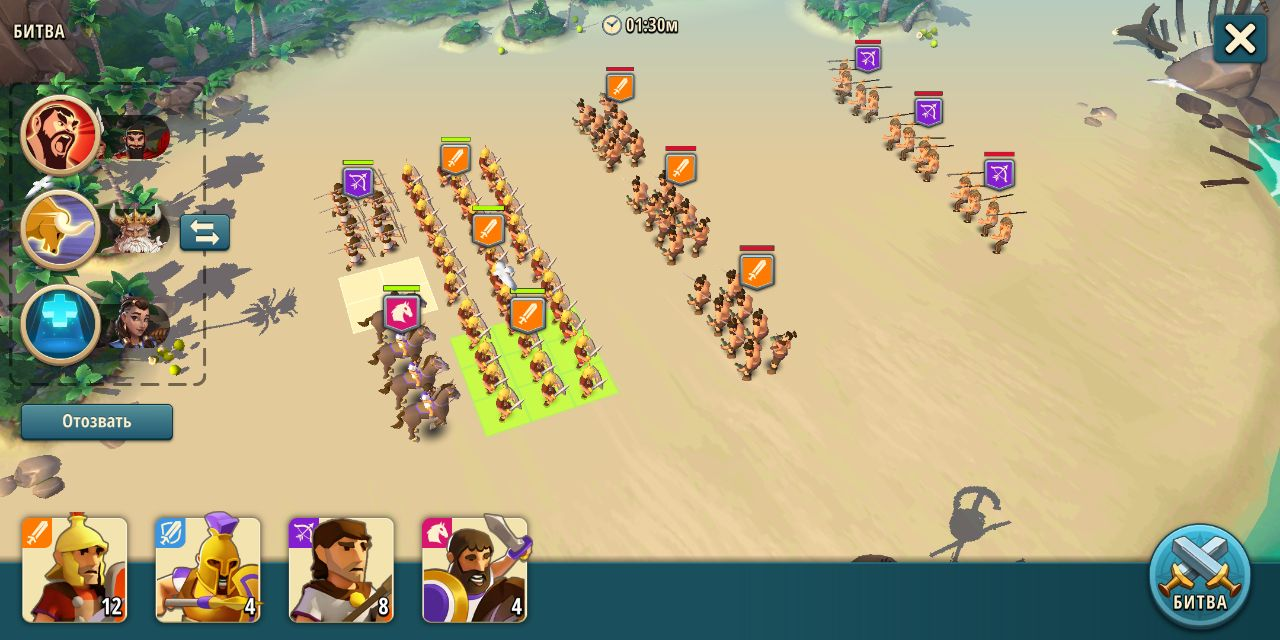
\includegraphics[width=0.75\linewidth]{./parts/media/TreasureHunt/21/sargon/photo_2022-04-06_18-11-33.jpg}} \\
	& Sargon &
	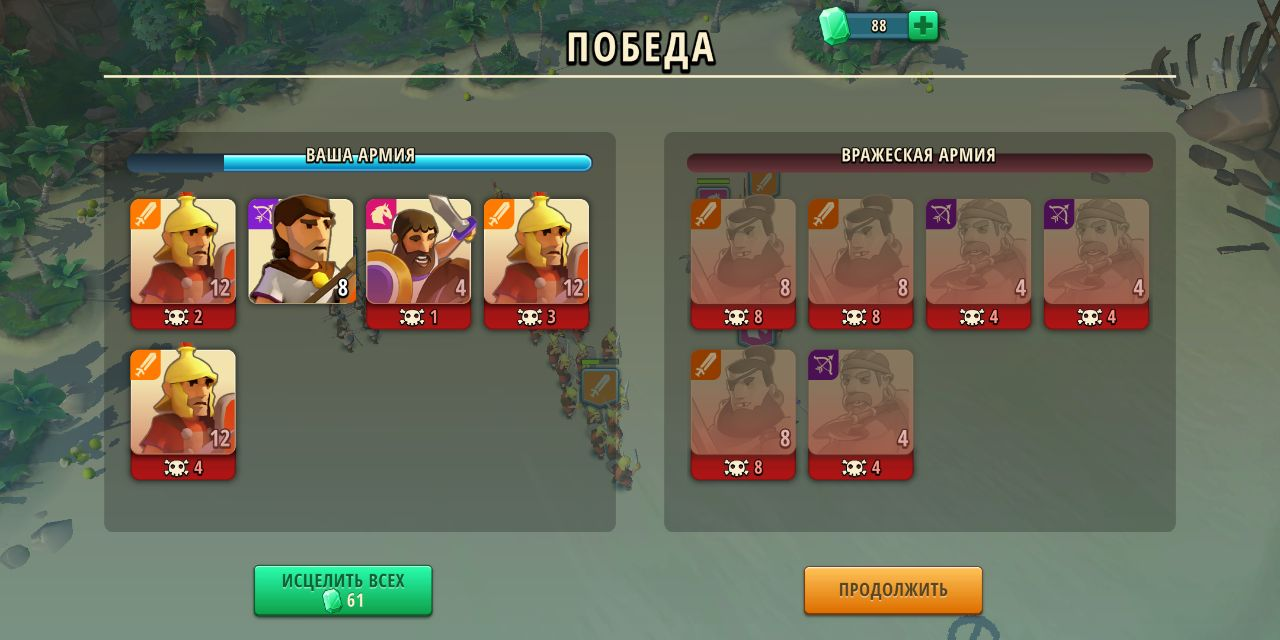
\includegraphics[width=0.75\linewidth]{./parts/media/TreasureHunt/21/sargon/photo_2022-04-06_18-11-59.jpg} \\
	\hline
	\multirow{8}{*}{22} & Sargon &
	\hypertarget{fight22}{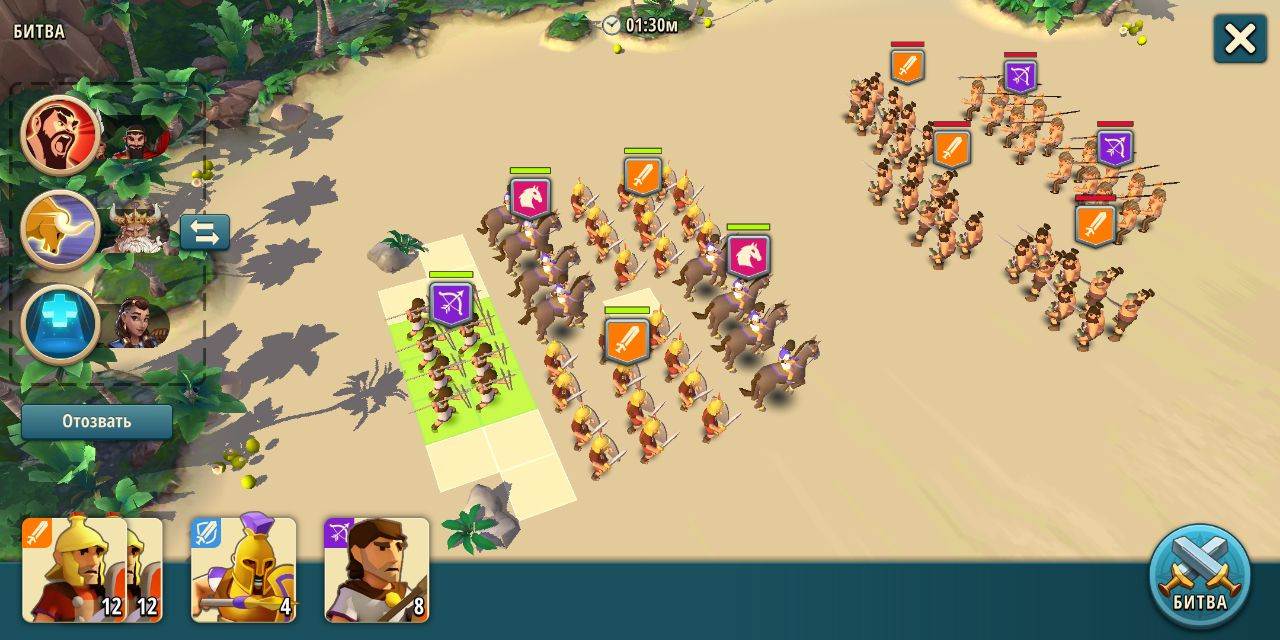
\includegraphics[width=0.75\linewidth]{./parts/media/TreasureHunt/22/sargon/photo_2022-04-06_18-12-03.jpg}} \\
	& Sargon &
	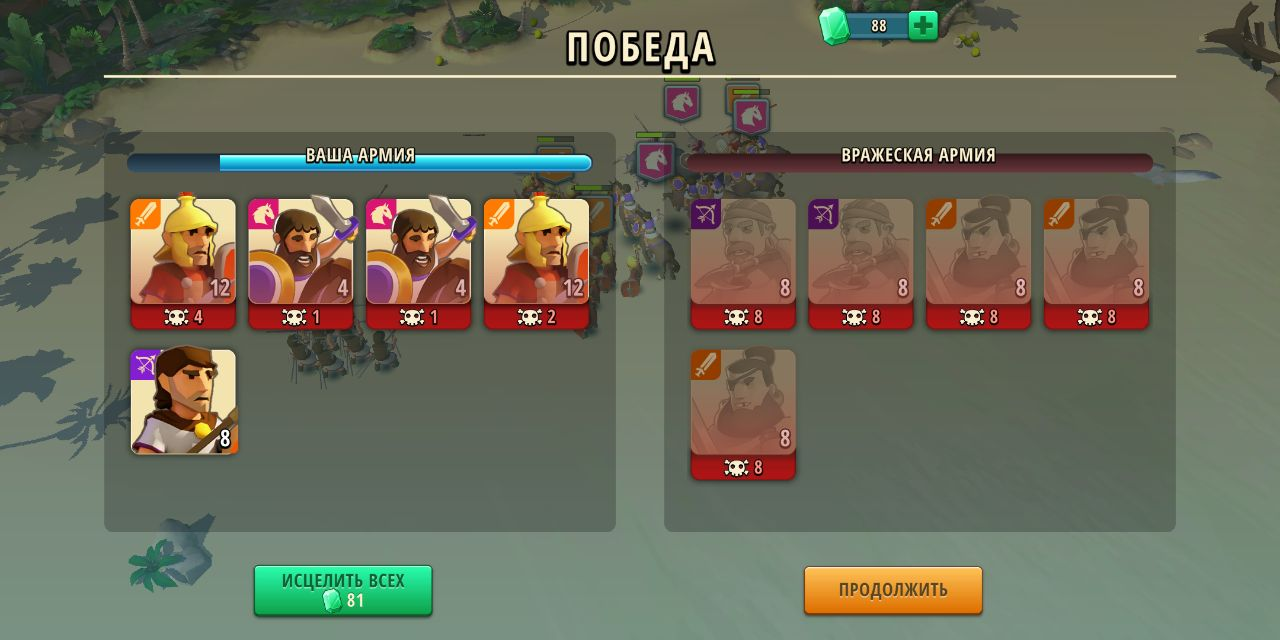
\includegraphics[width=0.75\linewidth]{./parts/media/TreasureHunt/22/sargon/photo_2022-04-06_18-12-13.jpg} \\
	\hline
	\multirow{8}{*}{22} & Preyton &
	\hypertarget{fight22}{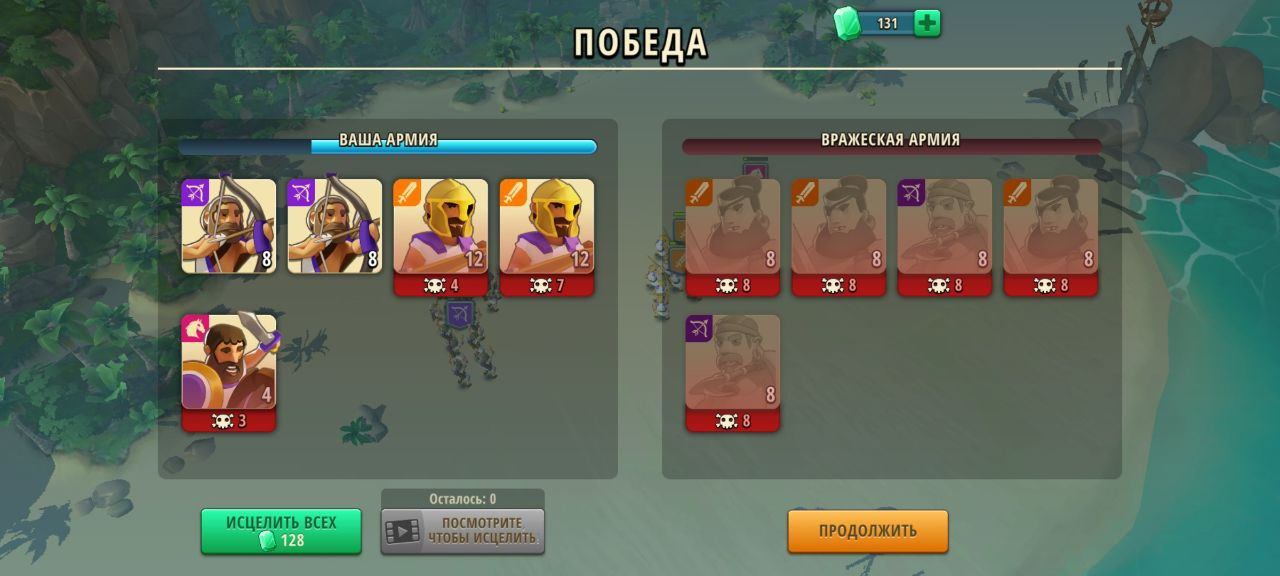
\includegraphics[width=0.75\linewidth]{./parts/media/TreasureHunt/22/Preyton/22..jpg}} \\
	& Preyton &
	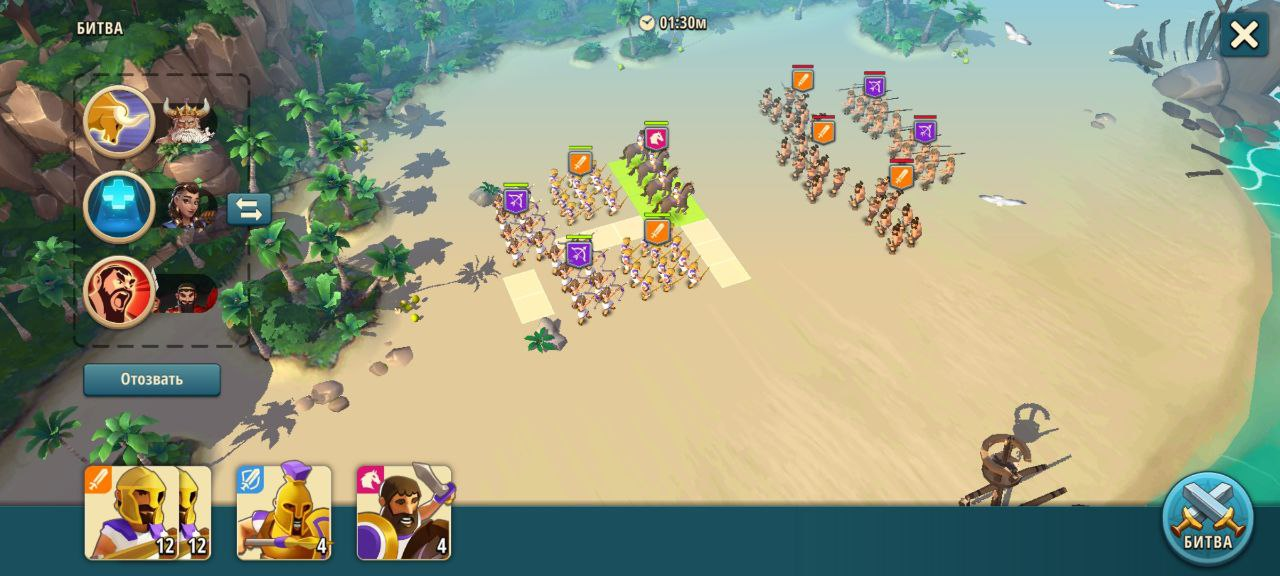
\includegraphics[width=0.75\linewidth]{./parts/media/TreasureHunt/22/Preyton/22.jpg} \\
	\hline
	\multirow{8}{*}{22} & Алексей &
	\hypertarget{fight22}{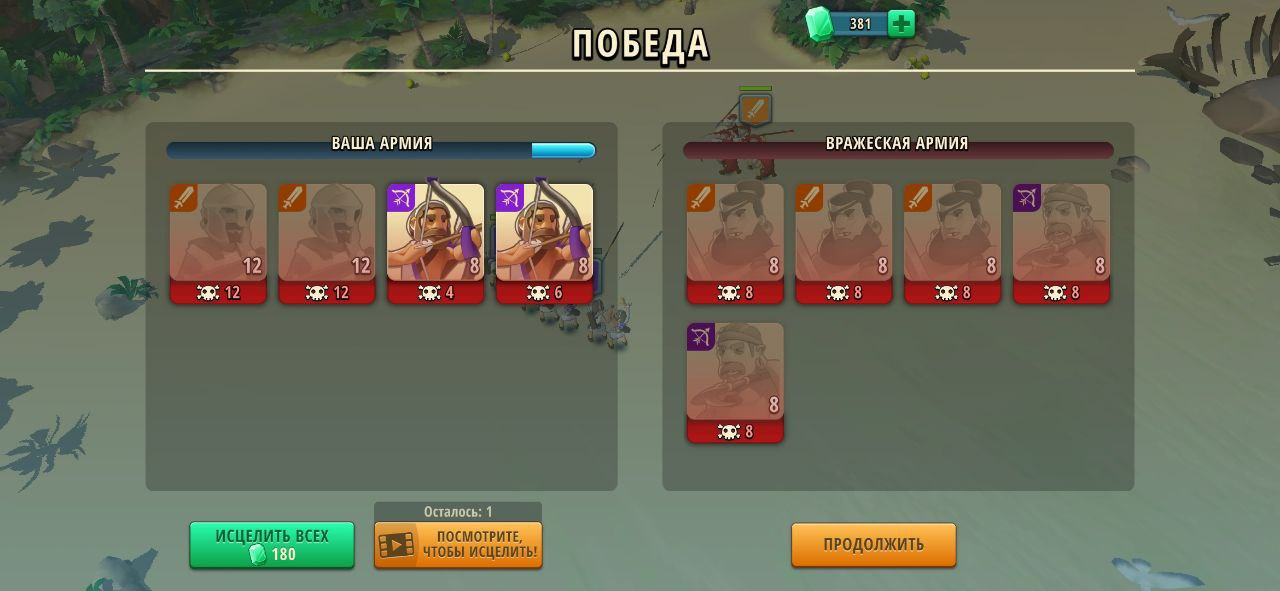
\includegraphics[width=0.75\linewidth]{./parts/media/TreasureHunt/22/alexey/photo_2022-04-13_16-28-21.jpg}} \\
	& Алексей &
	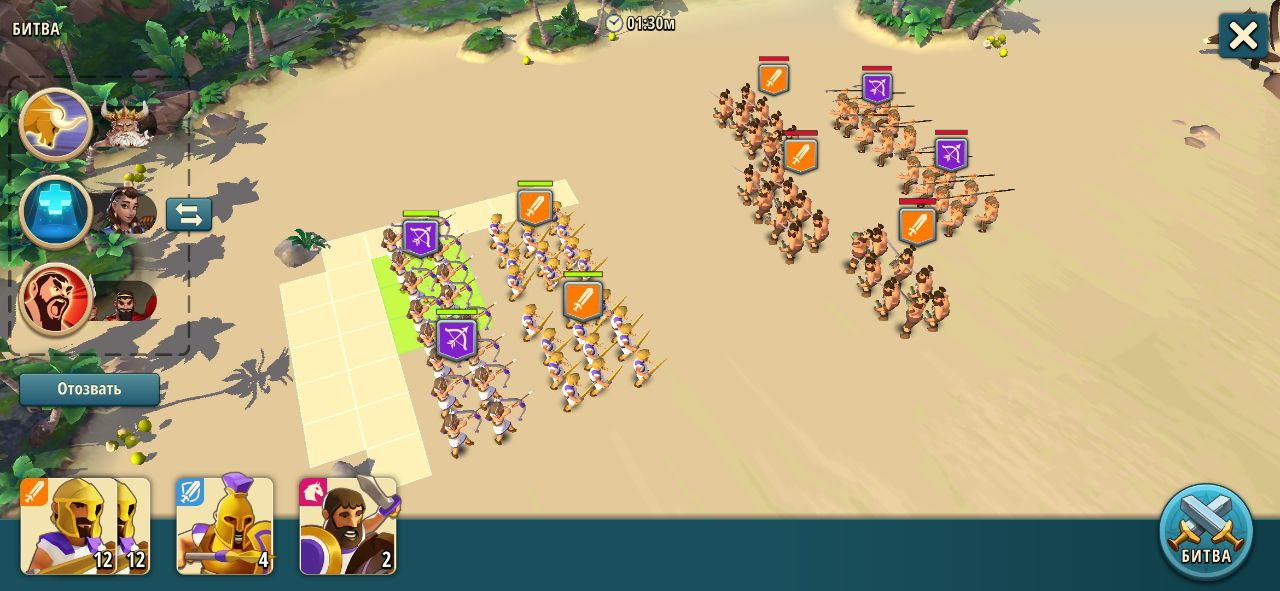
\includegraphics[width=0.75\linewidth]{./parts/media/TreasureHunt/22/alexey/photo_2022-04-13_16-28-31.jpg} \\
	\hline
	\multirow{8}{*}{22} & decoder &
	\hypertarget{fight22}{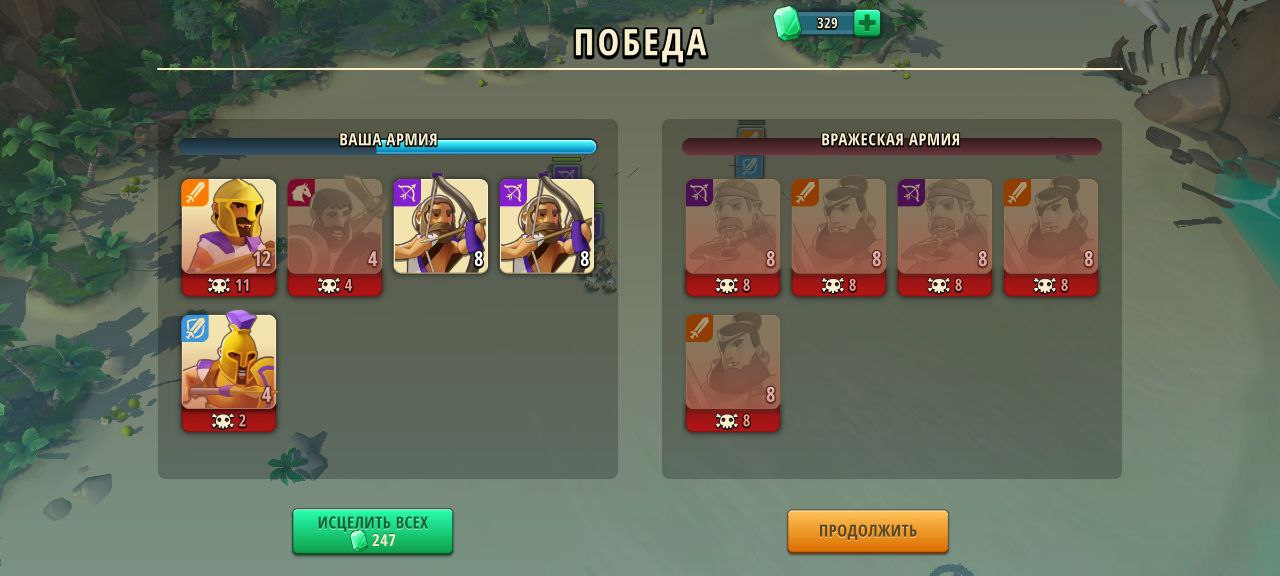
\includegraphics[width=0.75\linewidth]{./parts/media/TreasureHunt/22/decoder/photo_2022-04-13_16-27-45.jpg}} \\
	& decoder &
	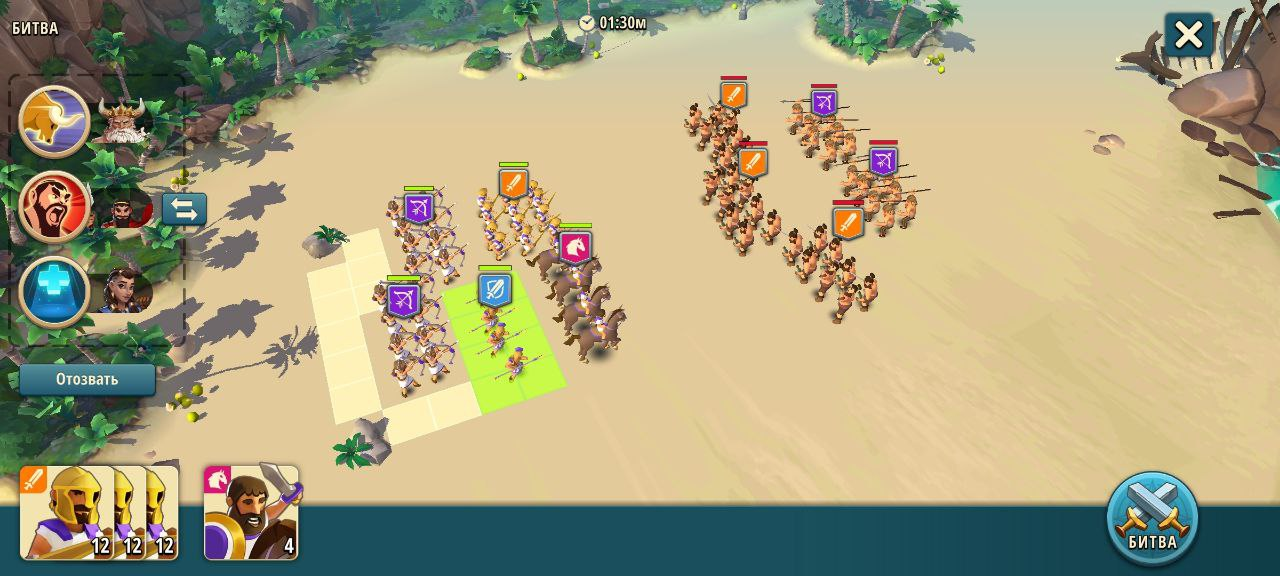
\includegraphics[width=0.75\linewidth]{./parts/media/TreasureHunt/22/decoder/photo_2022-04-13_16-27-22.jpg} \\
	\hline
	\multirow{8}{*}{23} & Sargon &
	\hypertarget{fight23}{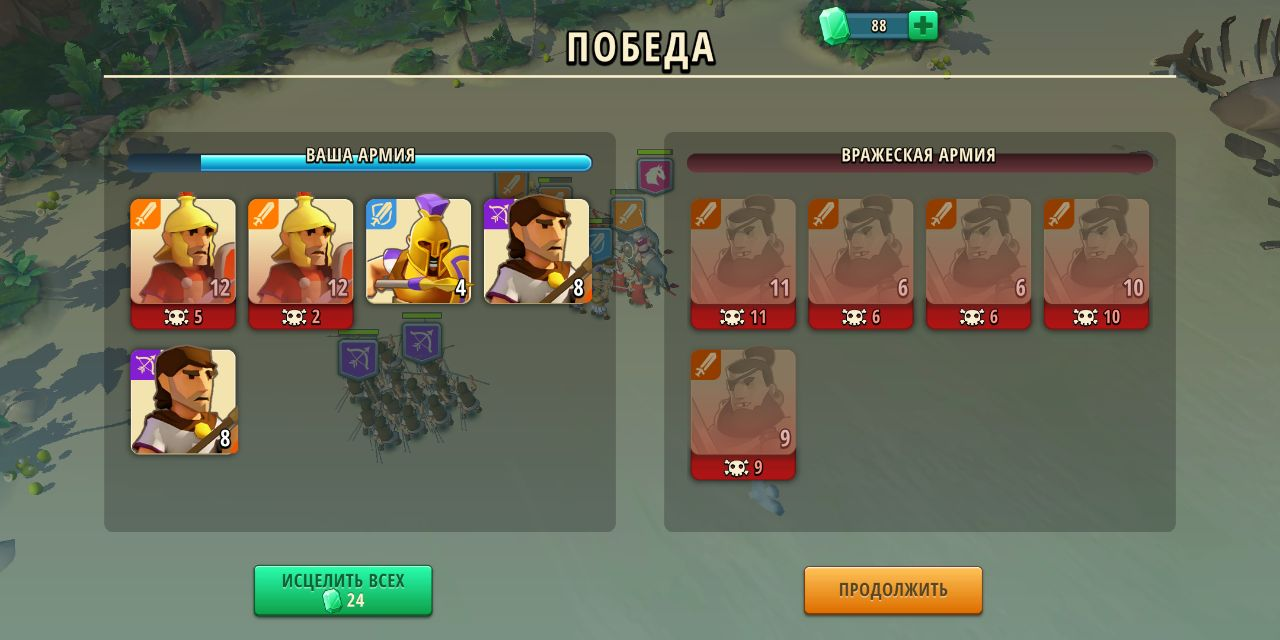
\includegraphics[width=0.75\linewidth]{./parts/media/TreasureHunt/23/sargon/photo_2022-04-06_18-12-26.jpg}} \\
	& Sargon &
	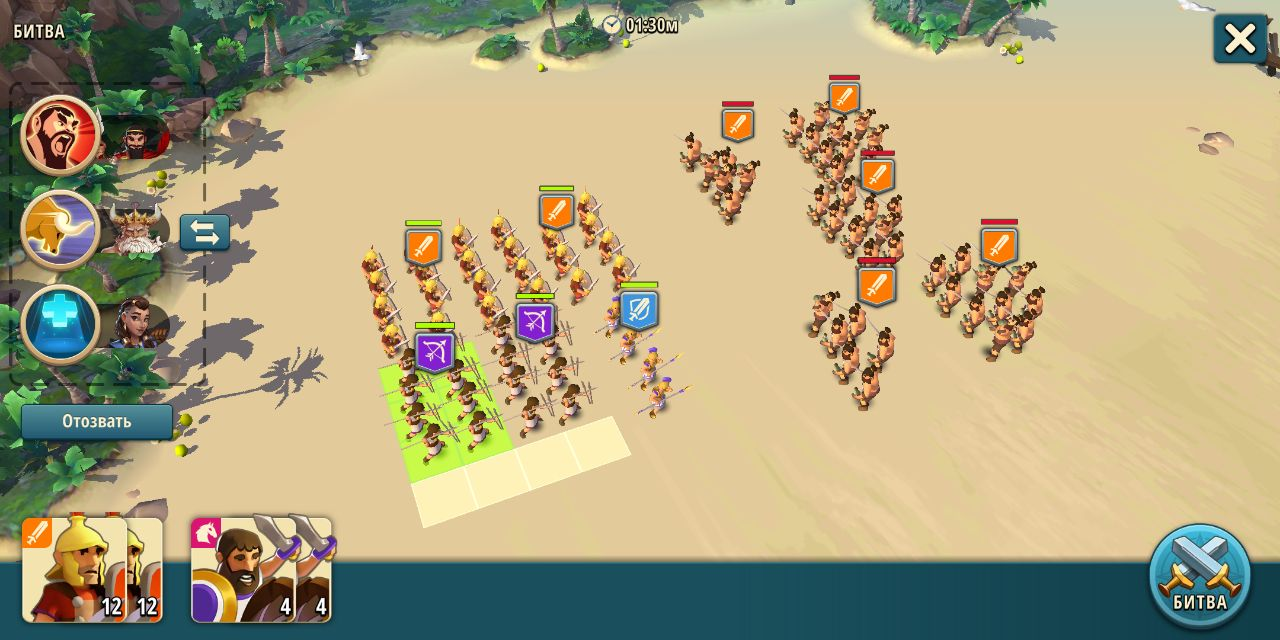
\includegraphics[width=0.75\linewidth]{./parts/media/TreasureHunt/23/sargon/photo_2022-04-06_18-12-18.jpg} \\
	\hline
	\multirow{8}{*}{23} & Preyton &
	\hypertarget{fight23}{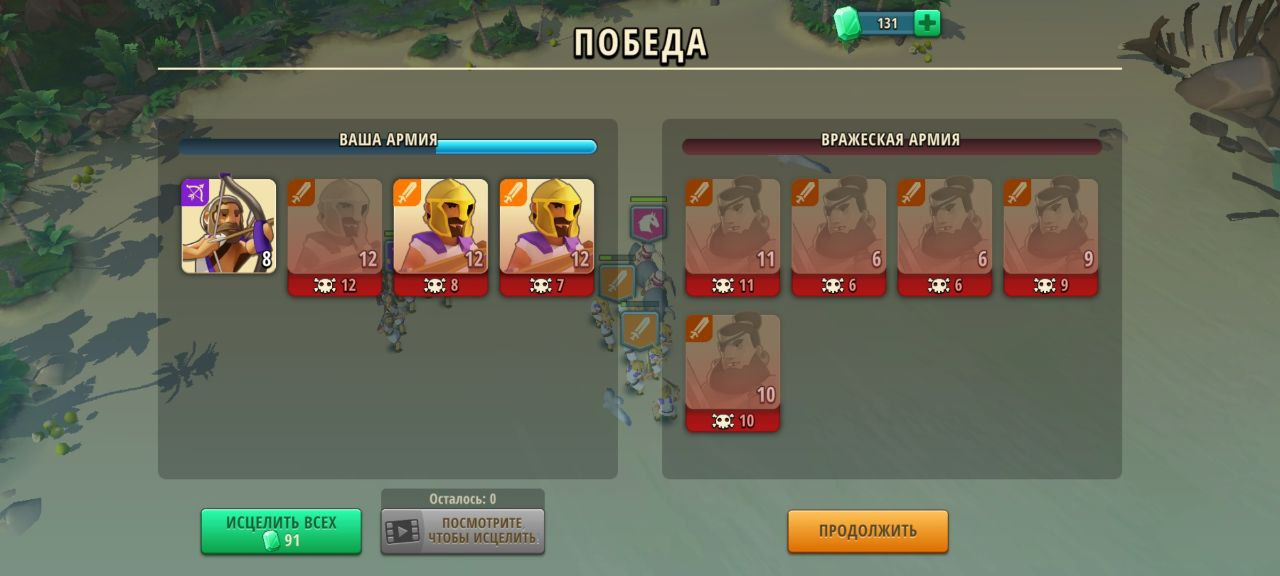
\includegraphics[width=0.75\linewidth]{./parts/media/TreasureHunt/23/Preyton/23..jpg}} \\
	& Preyton &
	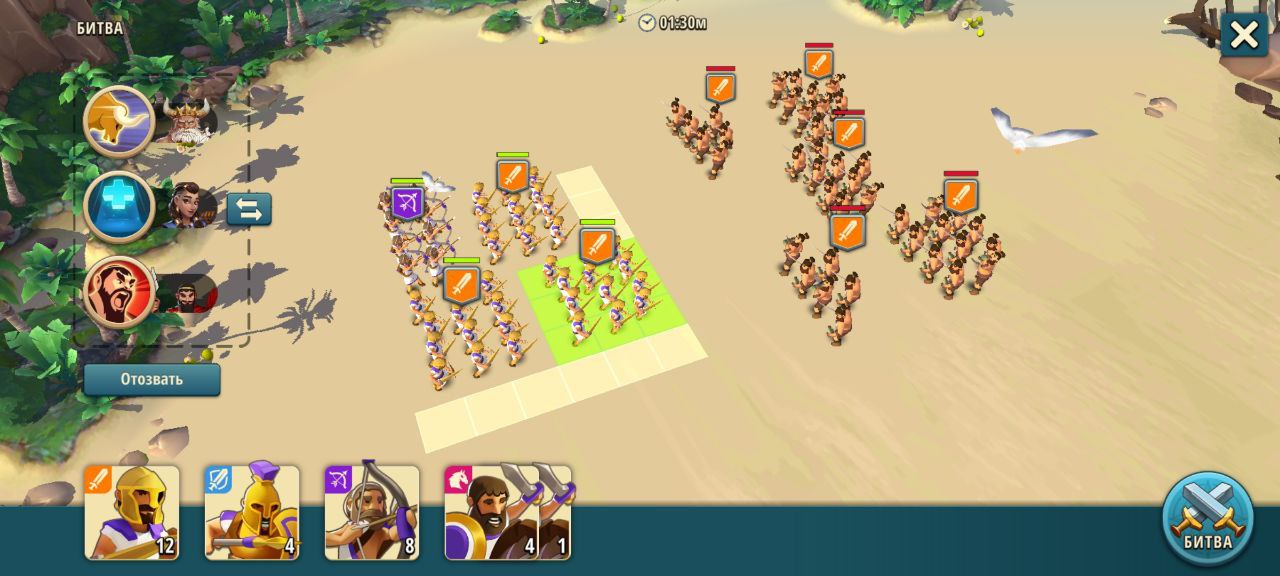
\includegraphics[width=0.75\linewidth]{./parts/media/TreasureHunt/23/Preyton/23.jpg} \\
	\hline
	\multirow{8}{*}{23} & Алексей &
	\hypertarget{fight23}{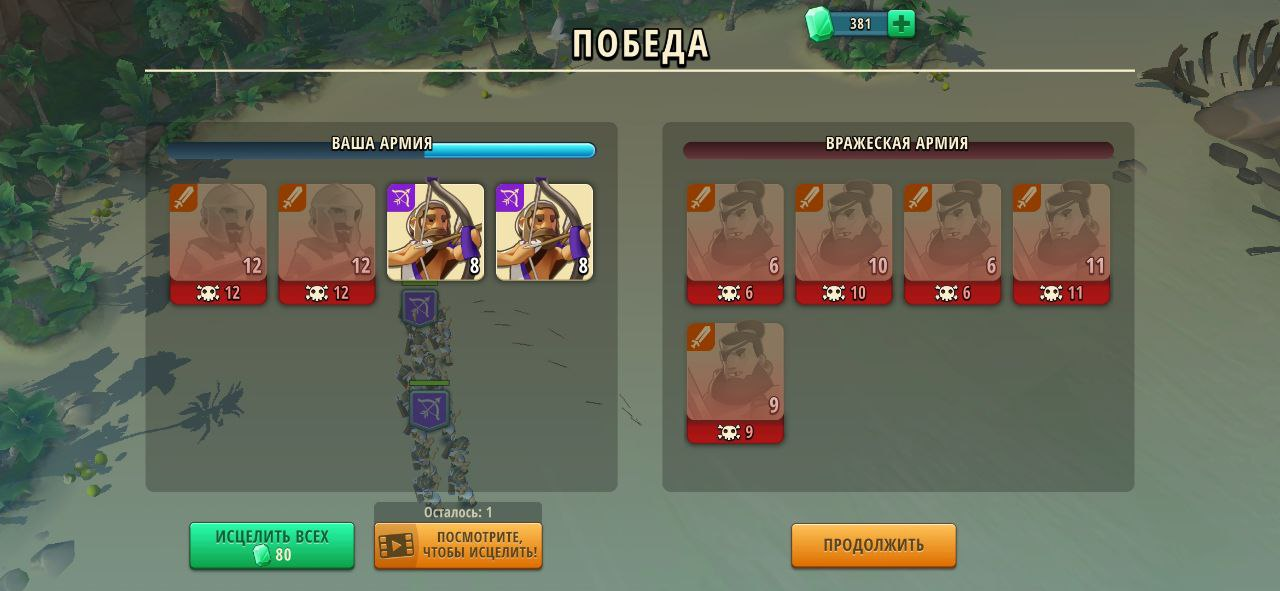
\includegraphics[width=0.75\linewidth]{./parts/media/TreasureHunt/23/alexey/photo_2022-04-13_19-01-32.jpg}} \\
	& Алексей &
	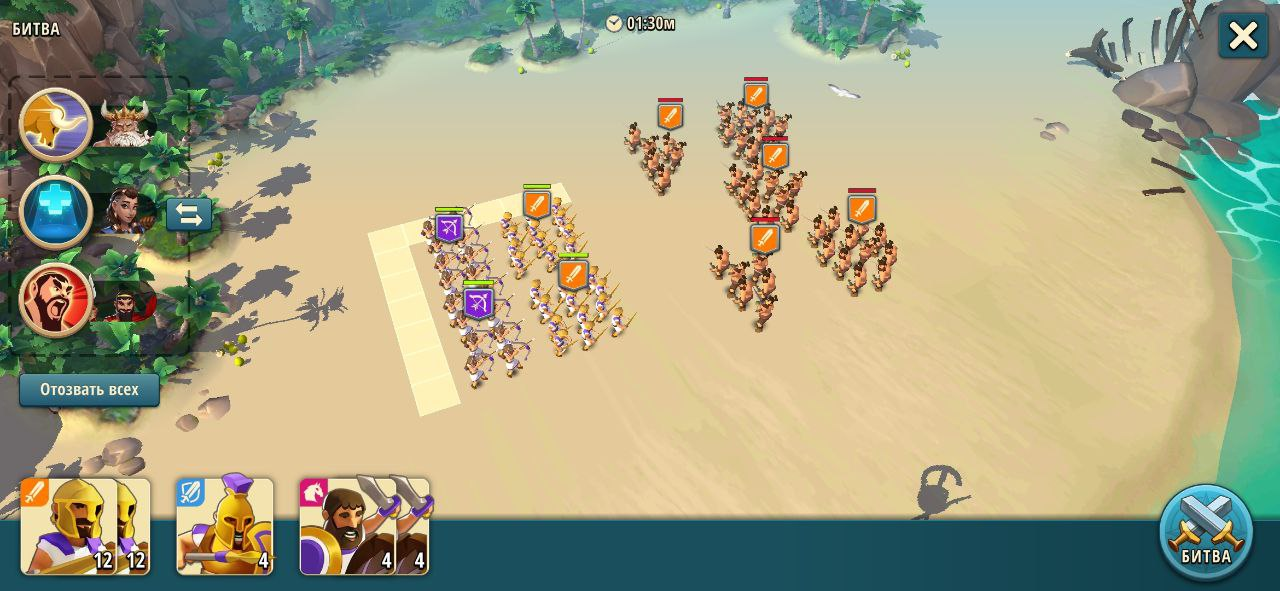
\includegraphics[width=0.75\linewidth]{./parts/media/TreasureHunt/23/alexey/photo_2022-04-13_19-01-54.jpg} \\
	\hline
	\multirow{8}{*}{23} & decoder &
	\hypertarget{fight23}{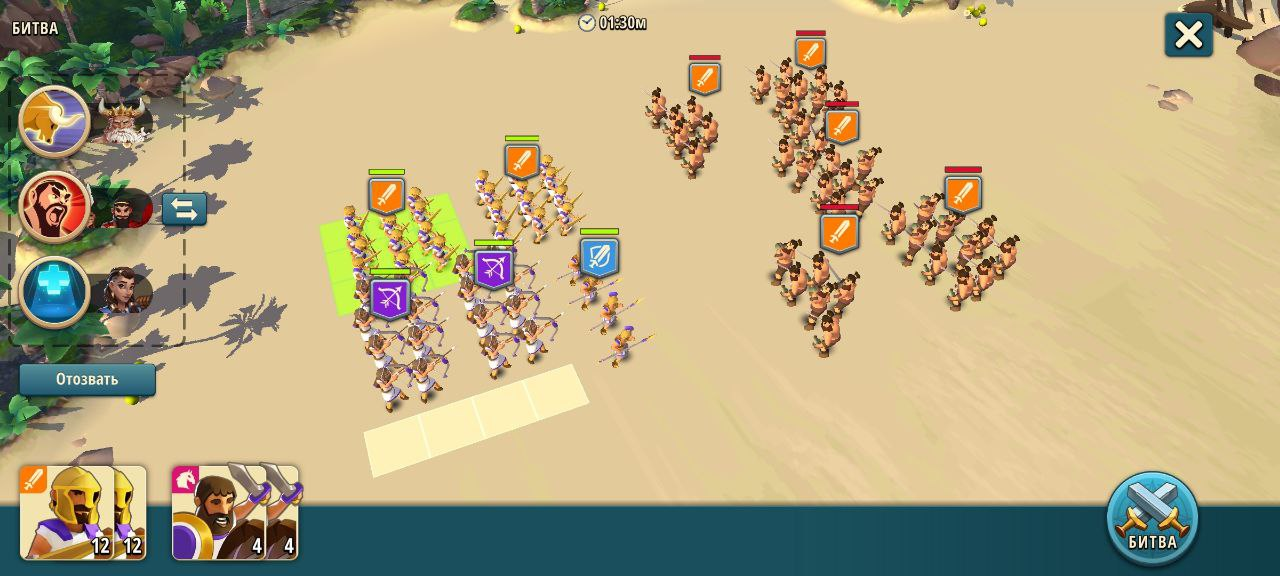
\includegraphics[width=0.75\linewidth]{./parts/media/TreasureHunt/23/decoder/photo_2022-04-13_16-27-58.jpg}} \\
	& decoder &
	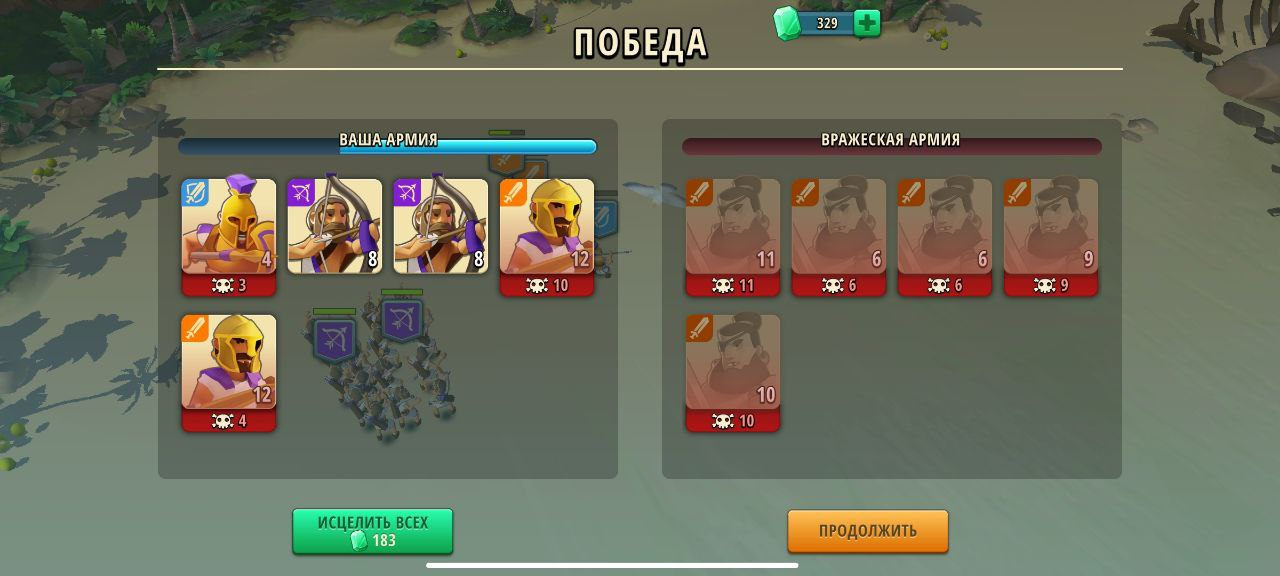
\includegraphics[width=0.75\linewidth]{./parts/media/TreasureHunt/23/decoder/photo_2022-04-13_16-28-07.jpg} \\
	\hline
	\multirow{6}{*}{24} & Preyton &
	\hypertarget{fight24}{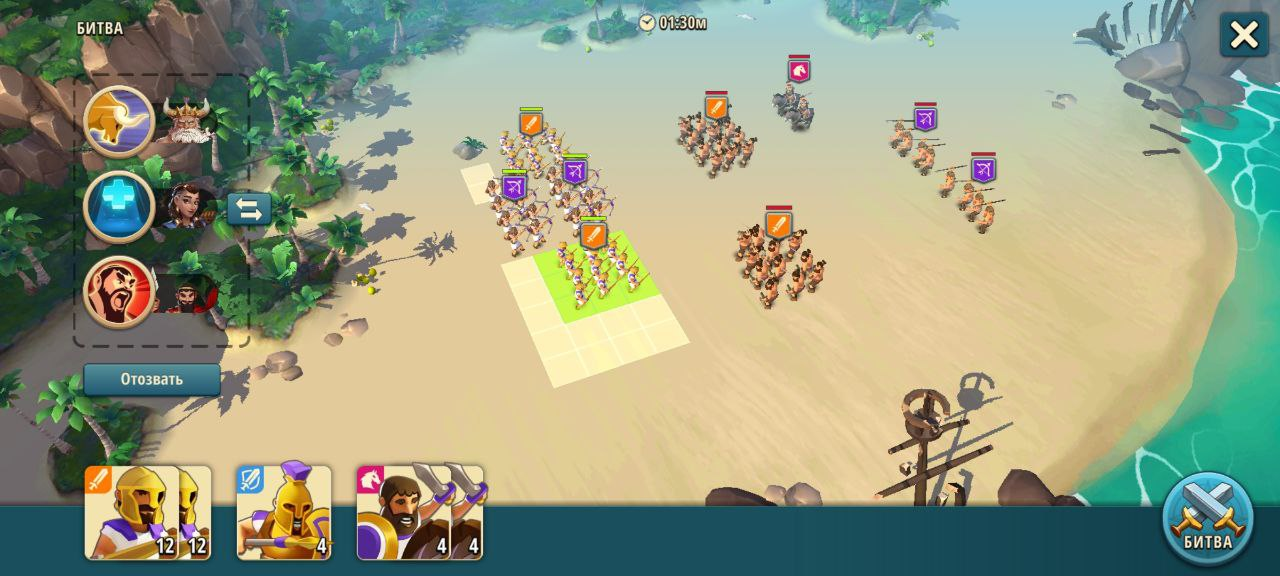
\includegraphics[width=0.75\linewidth]{./parts/media/TreasureHunt/24/Preyton/24.jpg}} \\
	& Preyton &
	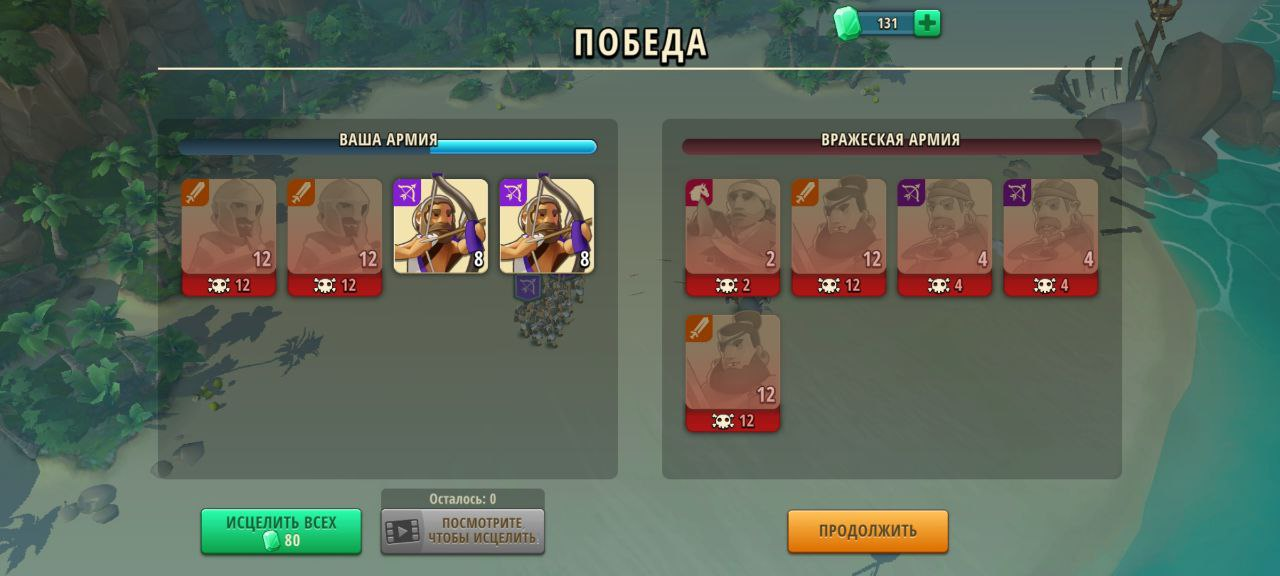
\includegraphics[width=0.75\linewidth]{./parts/media/TreasureHunt/24/Preyton/24..jpg} \\
	\hline
	\multirow{6}{*}{24} & Алексей &
	\hypertarget{fight24}{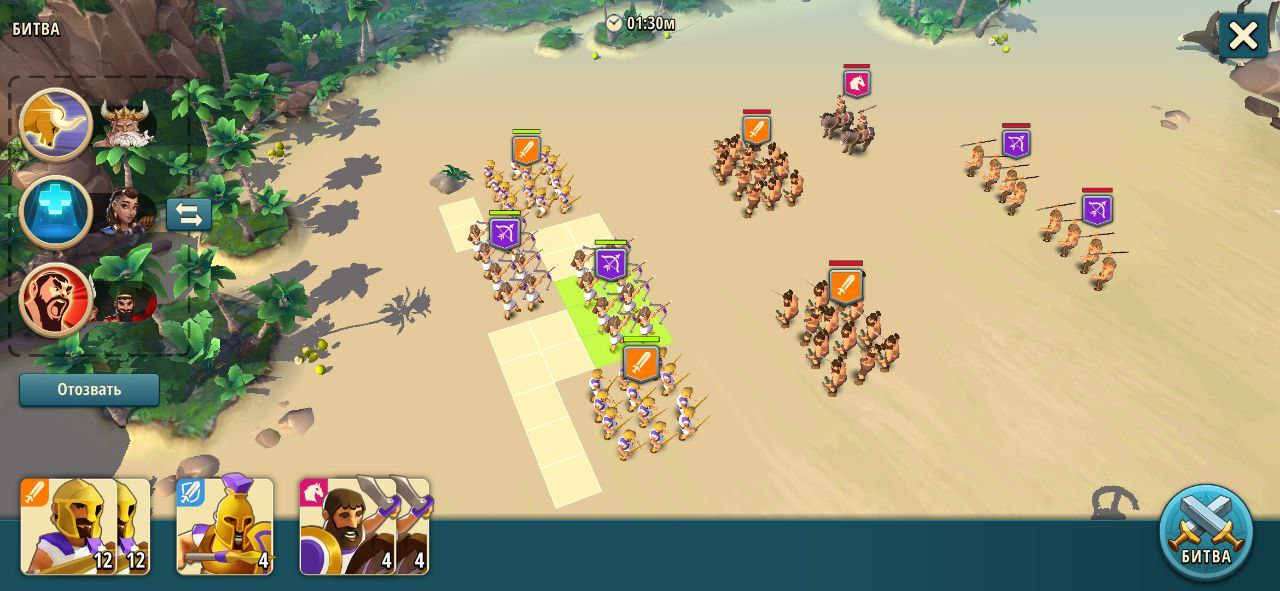
\includegraphics[width=0.75\linewidth]{./parts/media/TreasureHunt/24/alexey/photo_2022-04-13_19-02-08.jpg}} \\
	& Алексей &
	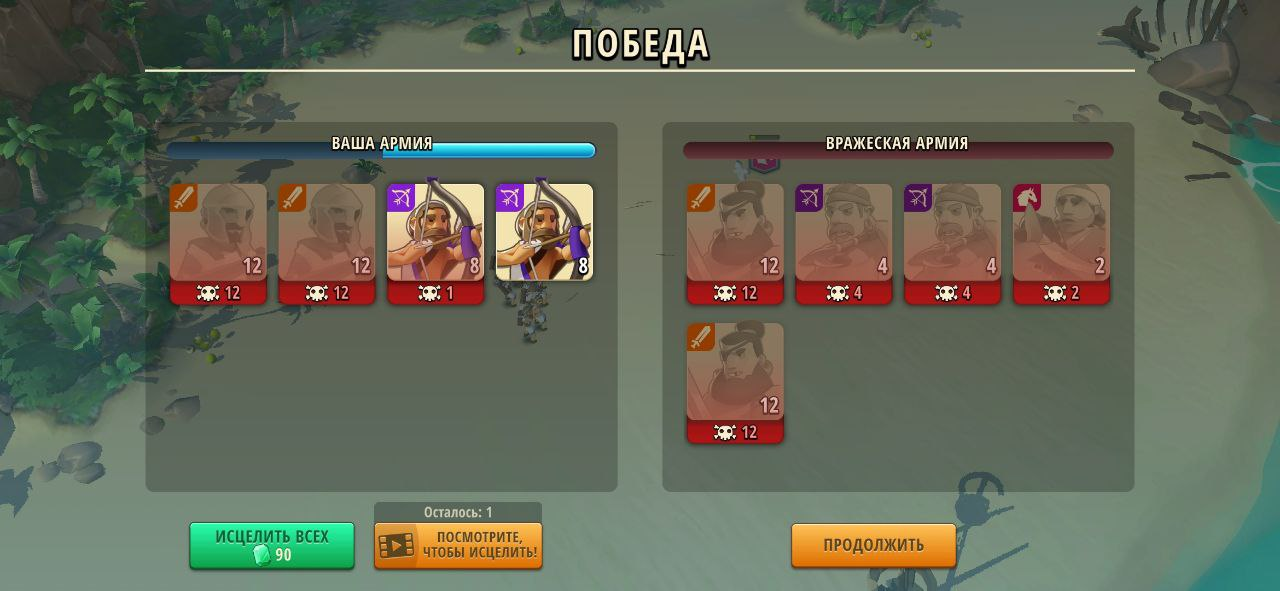
\includegraphics[width=0.75\linewidth]{./parts/media/TreasureHunt/24/alexey/photo_2022-04-13_19-01-59.jpg} \\
	\hline
	\multirow{6}{*}{24} & decoder &
	\hypertarget{fight24}{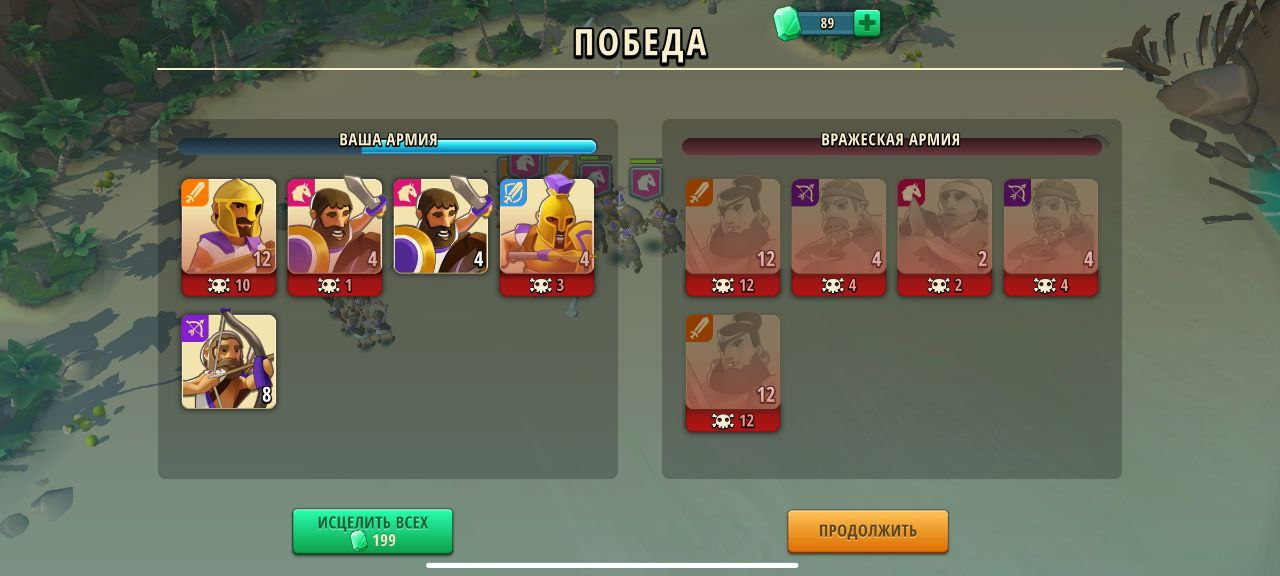
\includegraphics[width=0.75\linewidth]{./parts/media/TreasureHunt/24/decoder/photo_2022-04-06_18-10-13.jpg}} \\
	& decoder &
	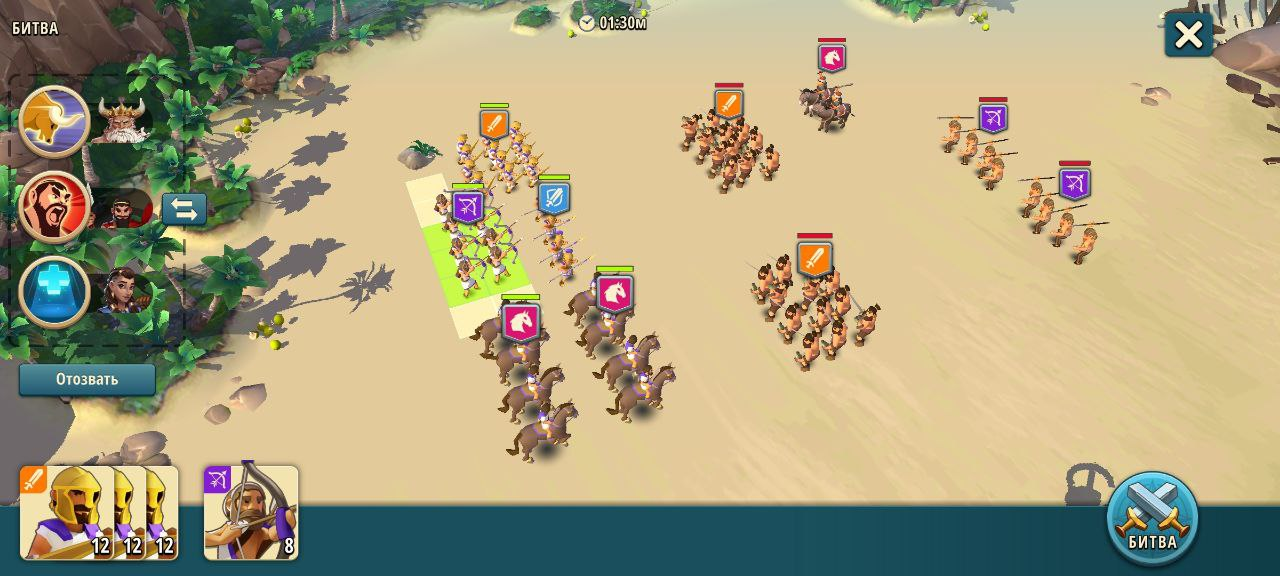
\includegraphics[width=0.75\linewidth]{./parts/media/TreasureHunt/24/decoder/photo_2022-04-06_18-10-02.jpg} \\
	\hline
	\multirow{14}{*}{25} & Sargon &
	\hypertarget{fight25}{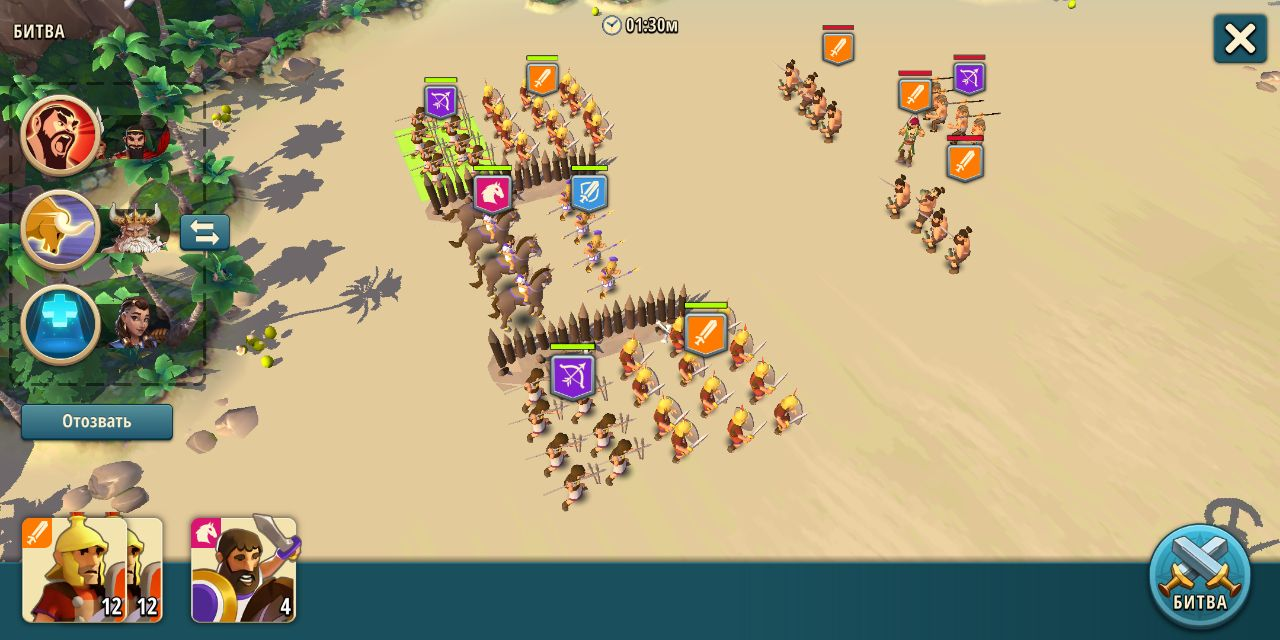
\includegraphics[width=0.75\linewidth]{./parts/media/TreasureHunt/25/sargon/photo_2022-04-07_09-58-16.jpg}} \\
	& Sargon &
	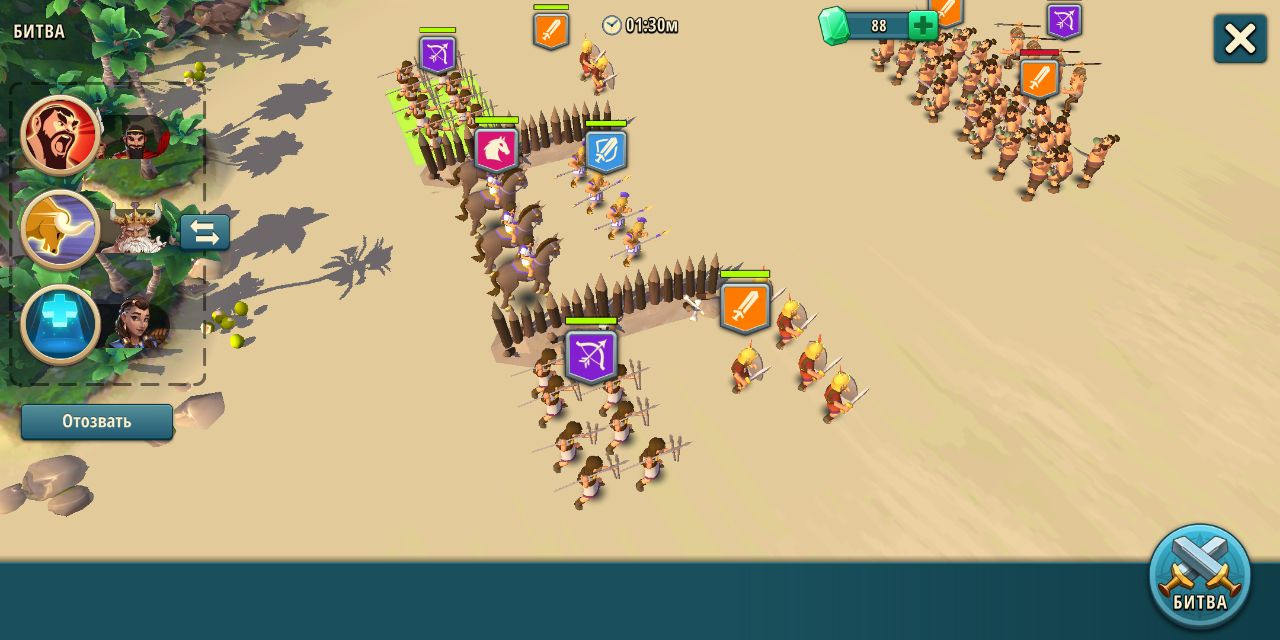
\includegraphics[width=0.75\linewidth]{./parts/media/TreasureHunt/25/sargon/photo_2022-04-07_09-58-31.jpg} \\
	& Sargon &
	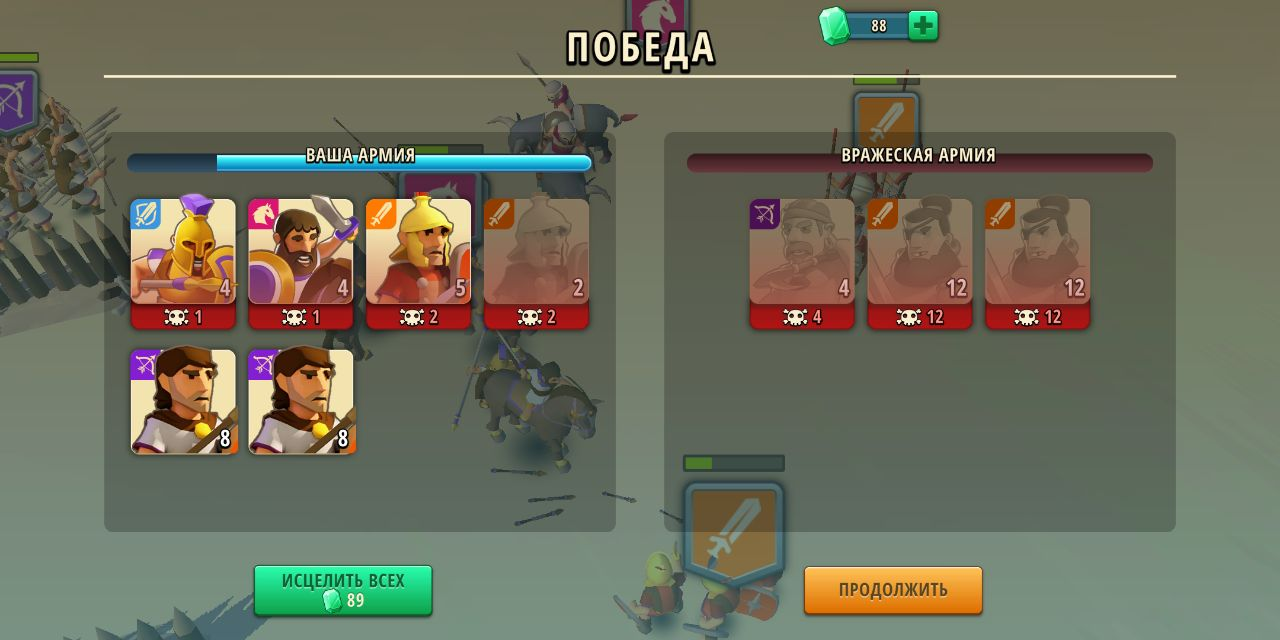
\includegraphics[width=0.75\linewidth]{./parts/media/TreasureHunt/25/sargon/photo_2022-04-07_09-58-35.jpg} \\
	& Sargon &
	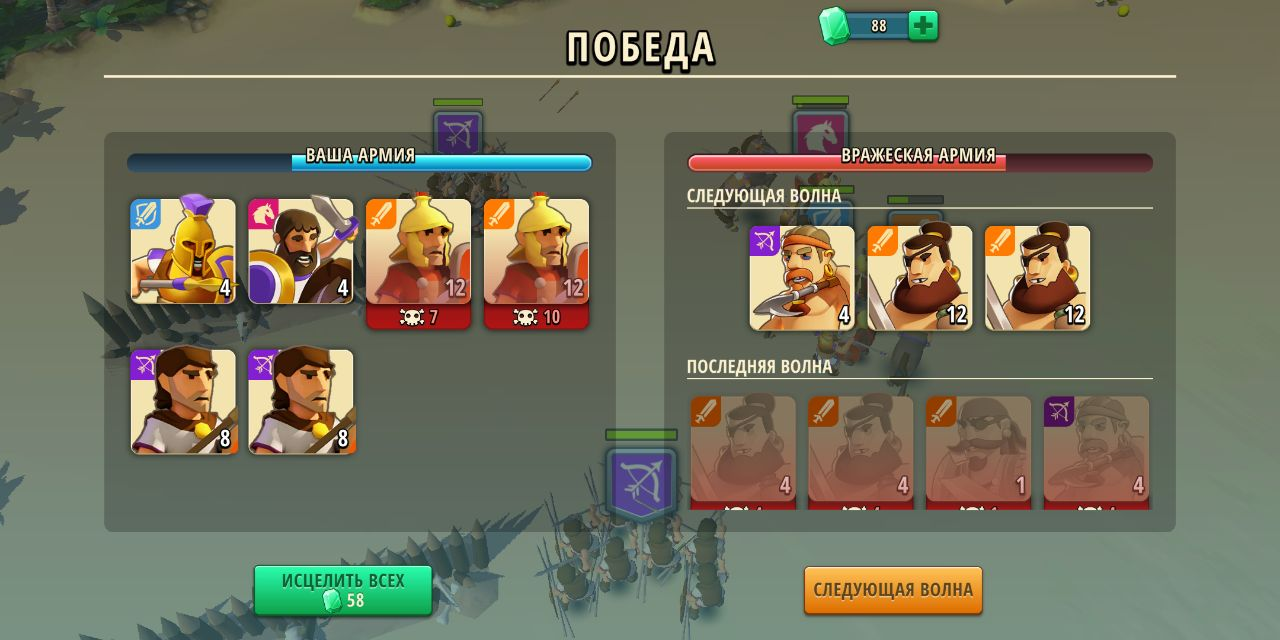
\includegraphics[width=0.75\linewidth]{./parts/media/TreasureHunt/25/sargon/photo_2022-04-07_09-58-27.jpg} \\
	\hline
	\multirow{14}{*}{25} & Preyton &
	\hypertarget{fight25}{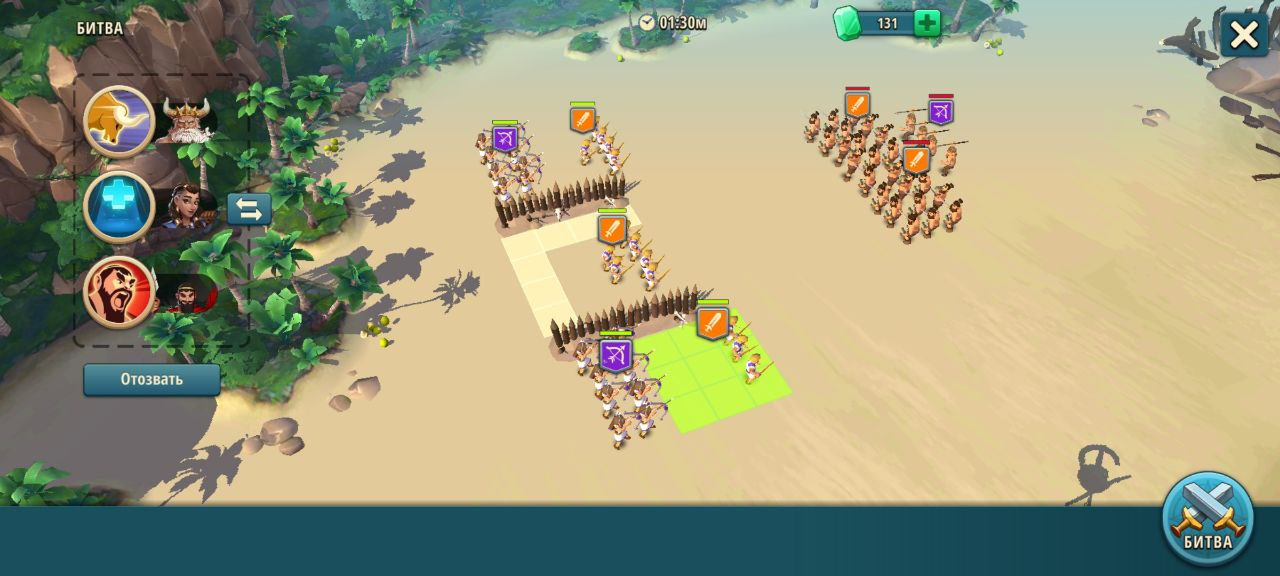
\includegraphics[width=0.75\linewidth]{./parts/media/TreasureHunt/25/Preyton/25.2.jpg}} \\
	& Preyton &
	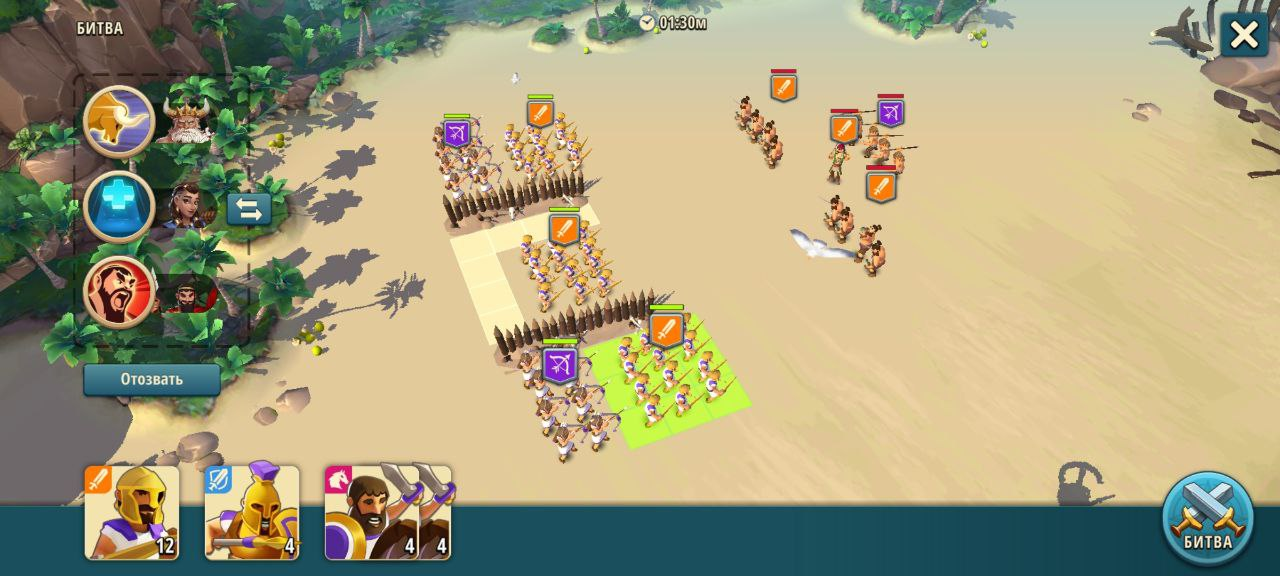
\includegraphics[width=0.75\linewidth]{./parts/media/TreasureHunt/25/Preyton/25.1.jpg} \\
	& Preyton &
	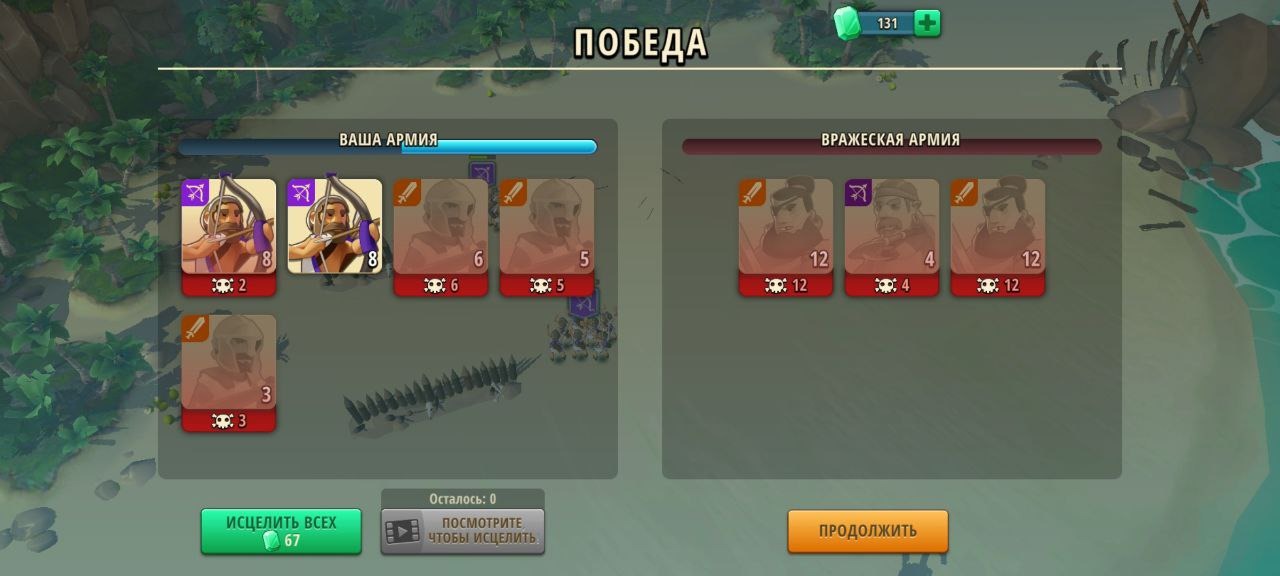
\includegraphics[width=0.75\linewidth]{./parts/media/TreasureHunt/25/Preyton/25_2.jpg} \\
	\hline
	\multirow{14}{*}{25} & Алексей &
	\hypertarget{fight25}{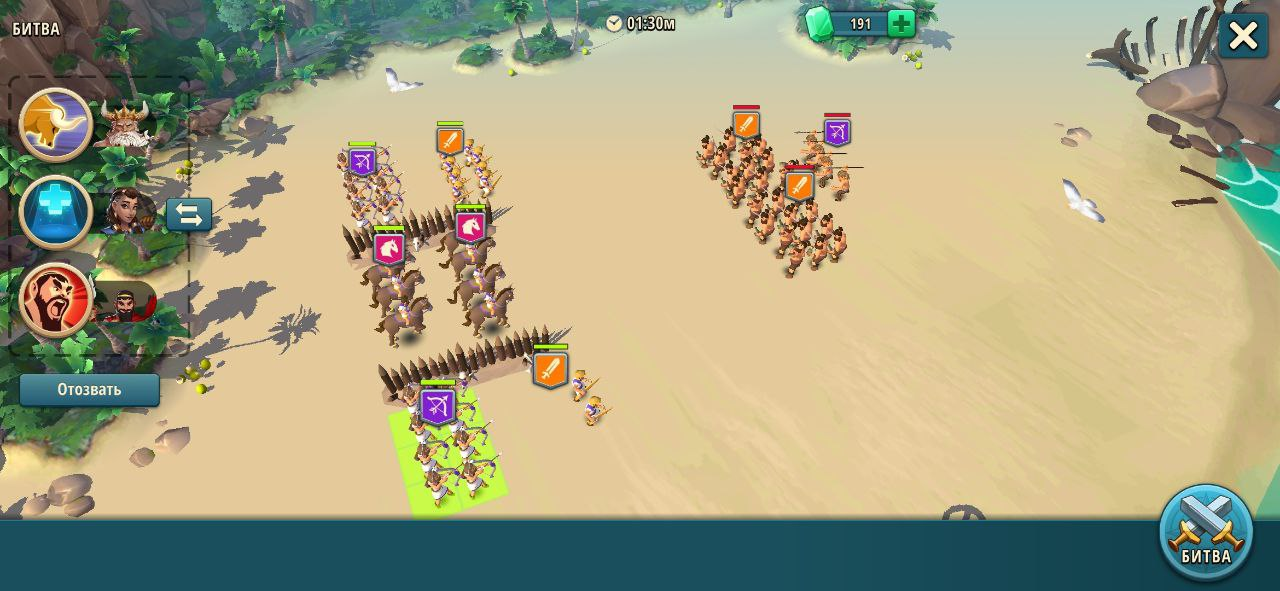
\includegraphics[width=0.75\linewidth]{./parts/media/TreasureHunt/25/alexey/photo_2022-04-07_10-09-19.jpg}} \\
	& Алексей &
	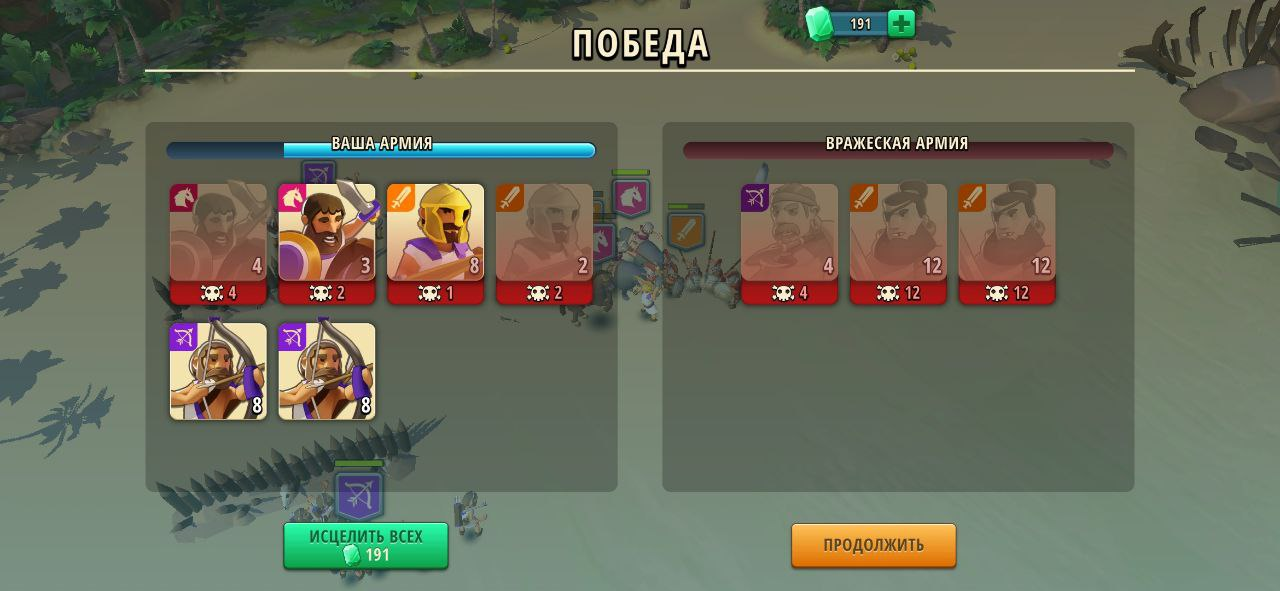
\includegraphics[width=0.75\linewidth]{./parts/media/TreasureHunt/25/alexey/photo_2022-04-07_10-09-24.jpg} \\
	& Алексей &
	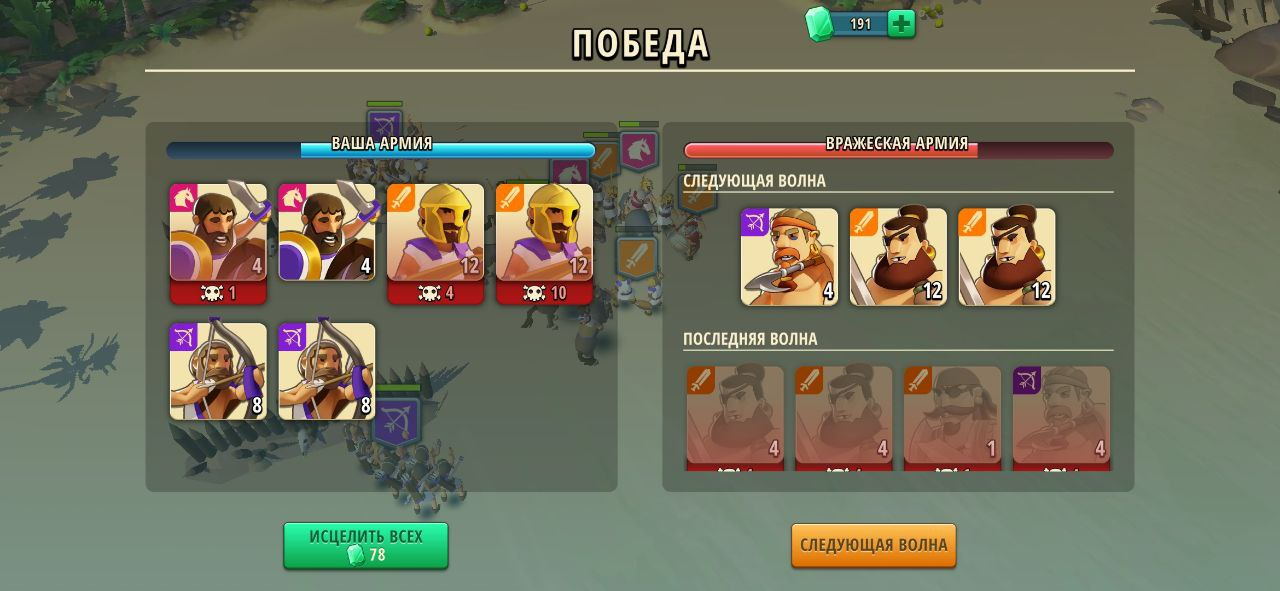
\includegraphics[width=0.75\linewidth]{./parts/media/TreasureHunt/25/alexey/photo_2022-04-07_10-09-08.jpg} \\
	\hline
	\multirow{14}{*}{25} & decoder &
	\hypertarget{fight25}{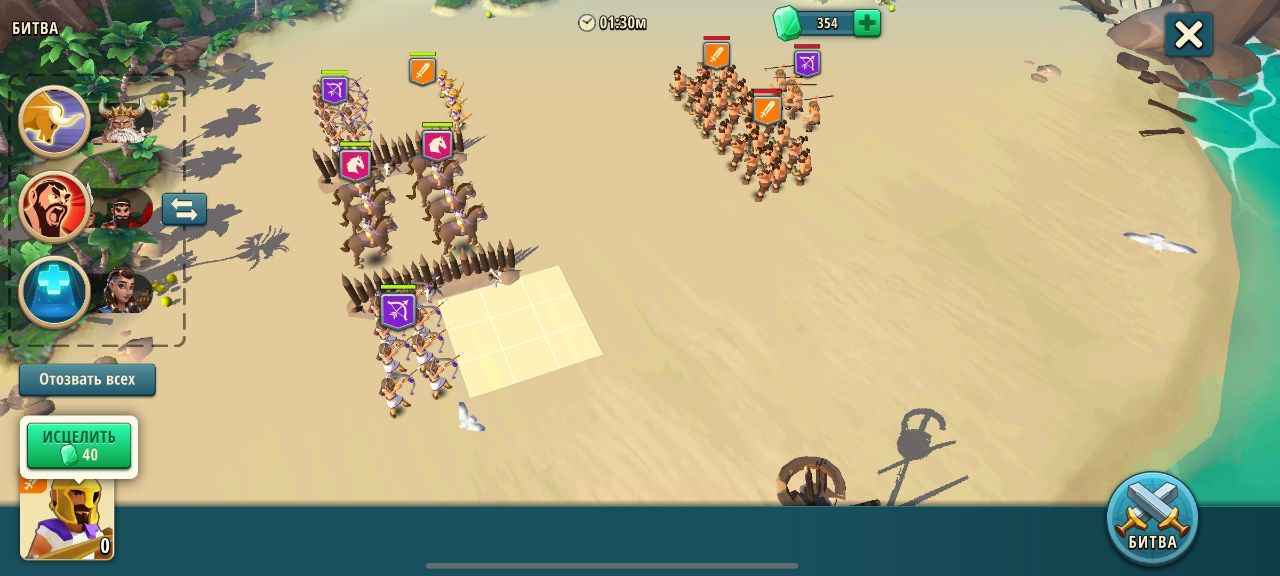
\includegraphics[width=0.75\linewidth]{./parts/media/TreasureHunt/25/decoder/photo_2022-04-13_16-38-53.jpg}} \\
	& decoder &
	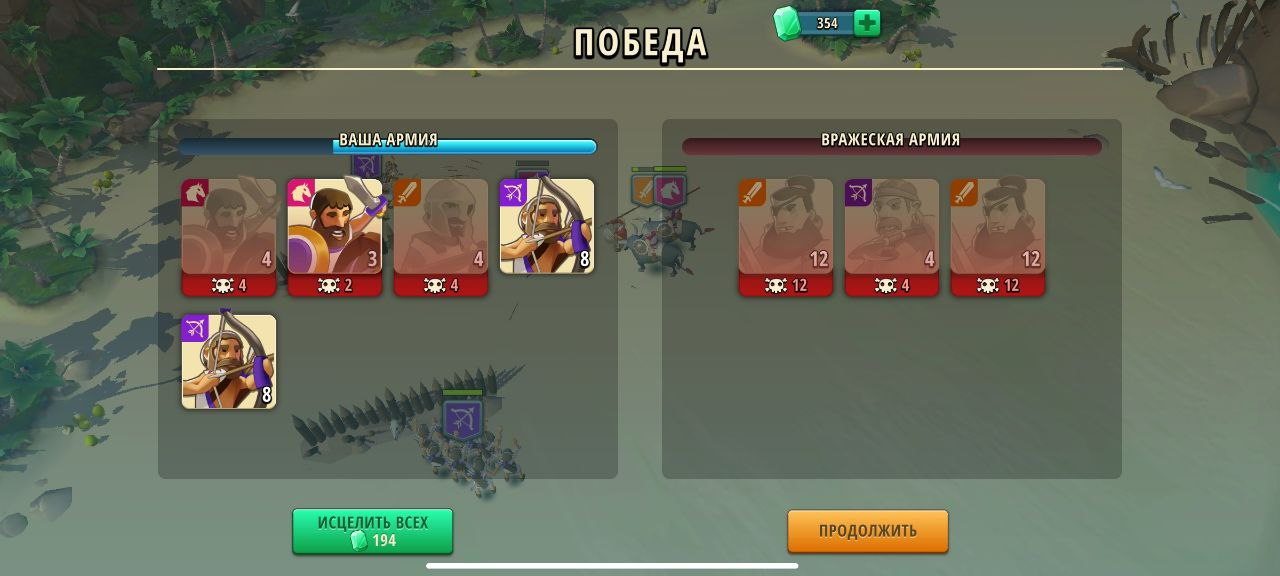
\includegraphics[width=0.75\linewidth]{./parts/media/TreasureHunt/25/decoder/photo_2022-04-13_16-38-58.jpg} \\
	& decoder &
	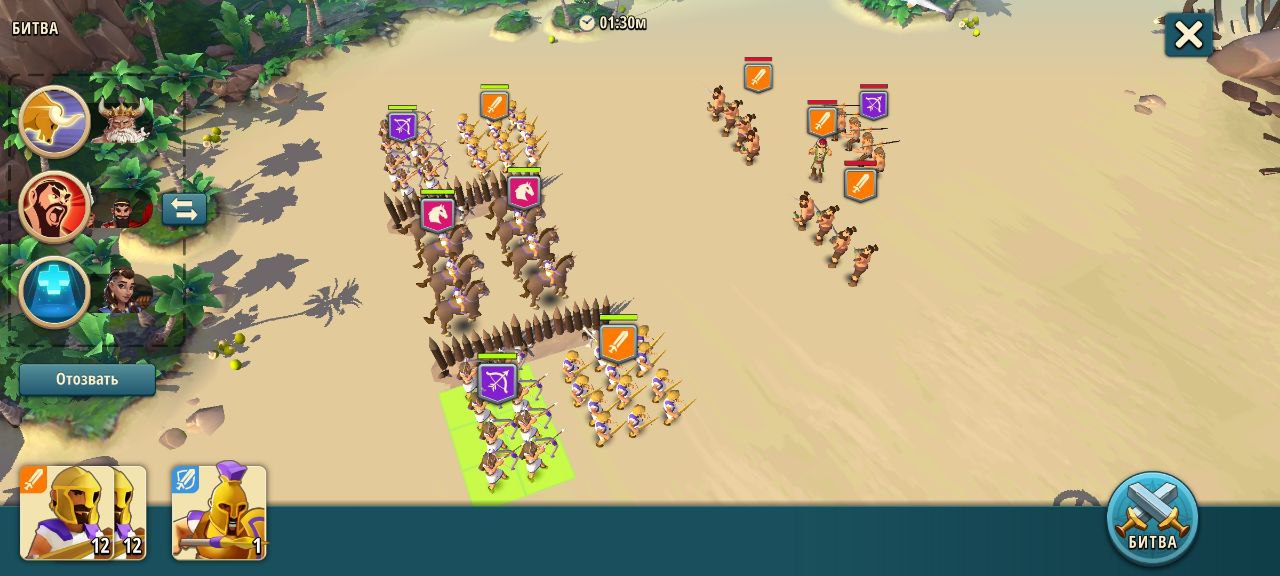
\includegraphics[width=0.75\linewidth]{./parts/media/TreasureHunt/25/decoder/photo_2022-04-13_16-38-30.jpg} \\
	& decoder &
	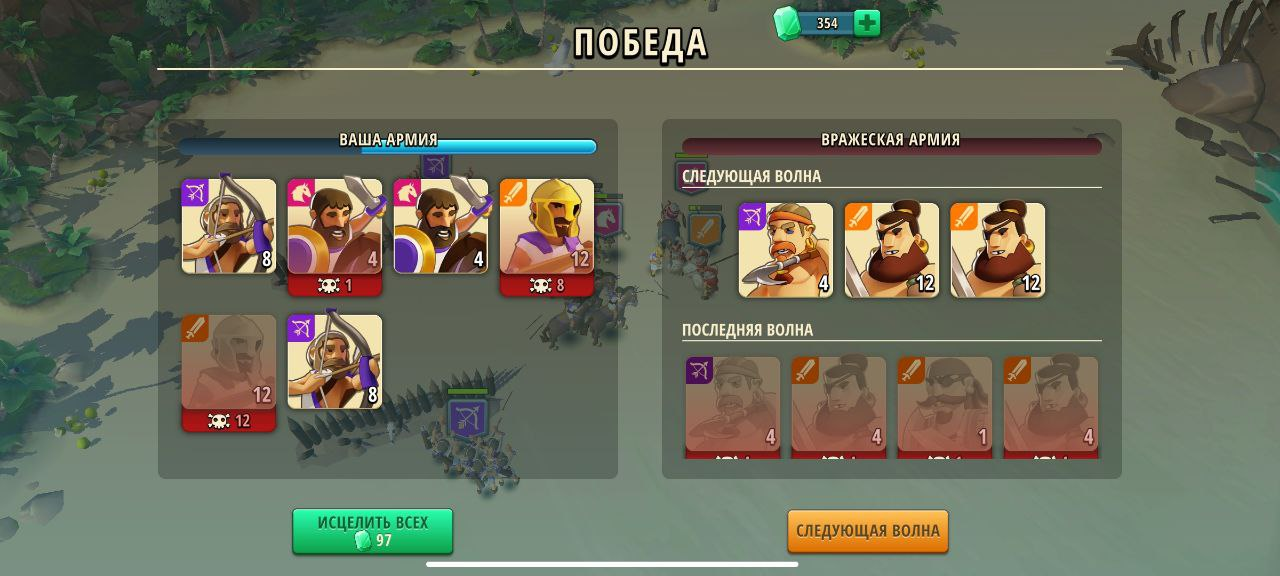
\includegraphics[width=0.75\linewidth]{./parts/media/TreasureHunt/25/decoder/photo_2022-04-13_16-38-45.jpg} \\
	\hline
	\multirow{6}{*}{26} & Preyton &
	\hypertarget{fight26}{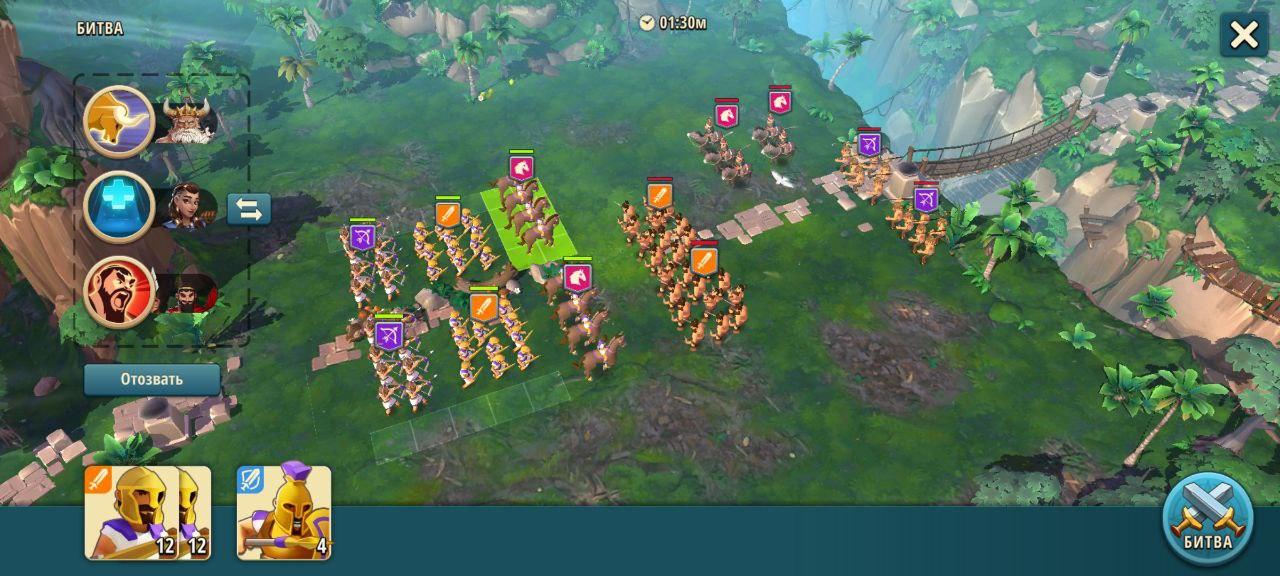
\includegraphics[width=0.75\linewidth]{./parts/media/TreasureHunt/26/Preyton/26.jpg}} \\
	& Preyton &
	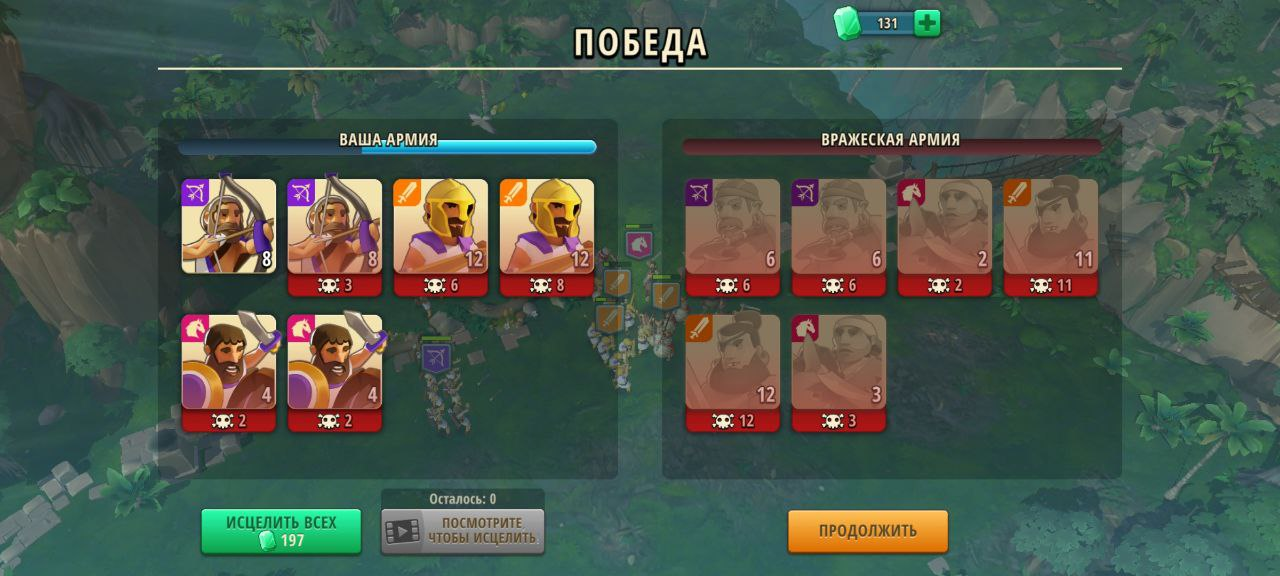
\includegraphics[width=0.75\linewidth]{./parts/media/TreasureHunt/26/Preyton/26..jpg} \\
	\hline
	\multirow{6}{*}{26} & Алексей &
	\hypertarget{fight26}{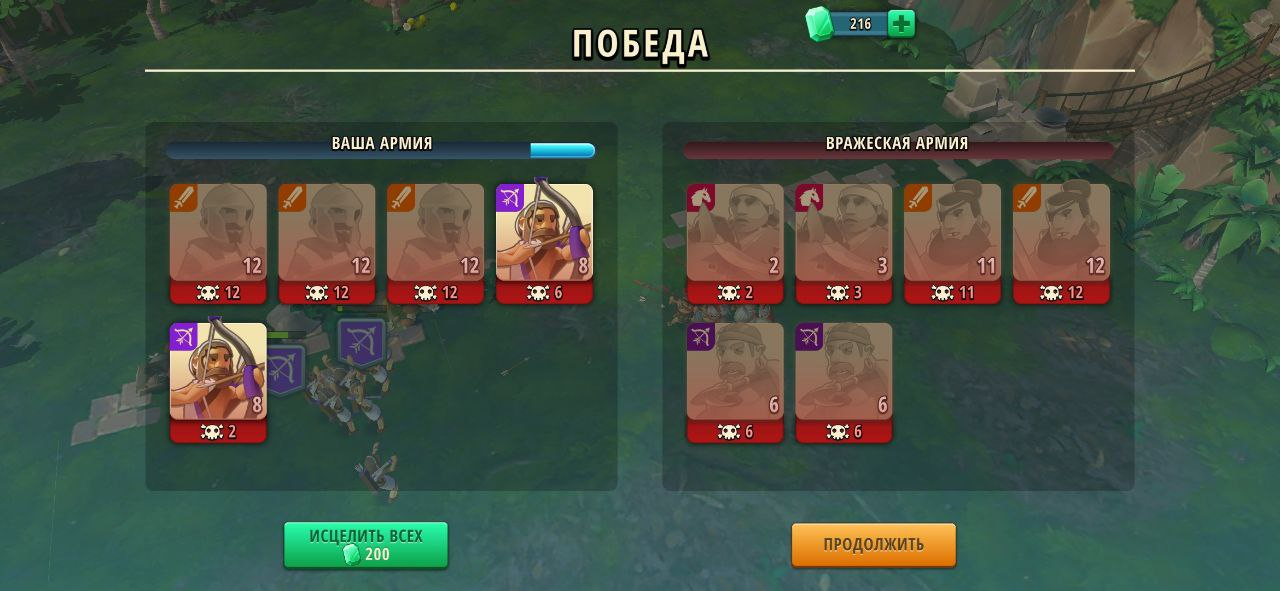
\includegraphics[width=0.75\linewidth]{./parts/media/TreasureHunt/26/alexey/photo_2022-04-07_10-09-39.jpg}} \\
	& Алексей &
	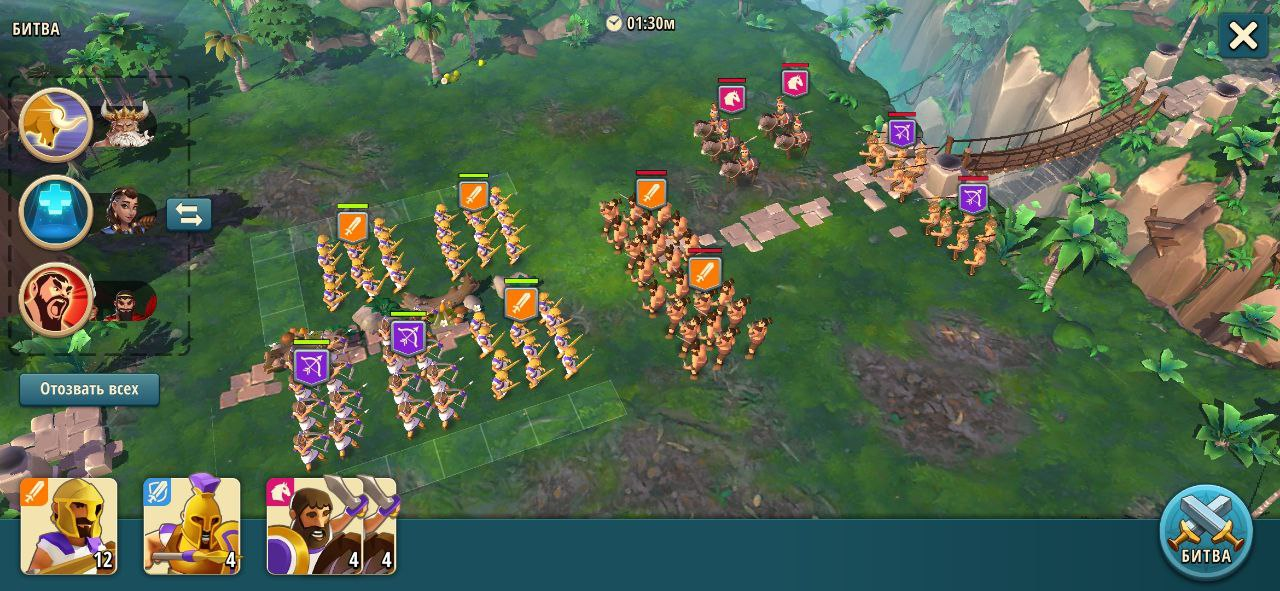
\includegraphics[width=0.75\linewidth]{./parts/media/TreasureHunt/26/alexey/photo_2022-04-07_10-09-28.jpg} \\
	\hline
	\multirow{6}{*}{26} & decoder &
	\hypertarget{fight26}{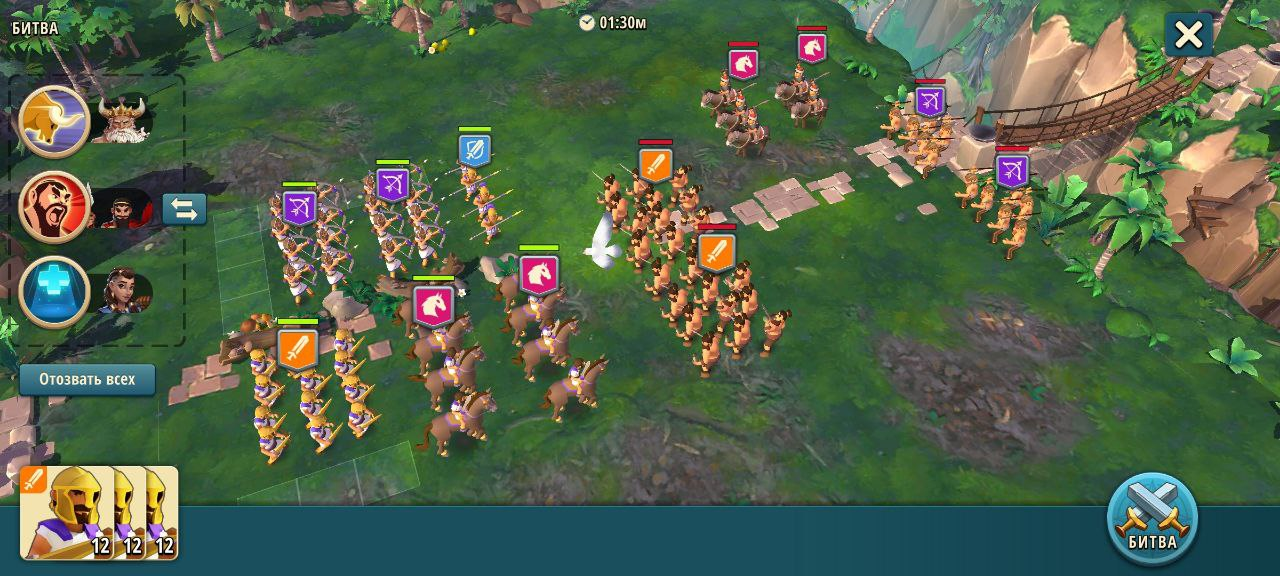
\includegraphics[width=0.75\linewidth]{./parts/media/TreasureHunt/26/decoder/photo_2022-04-06_18-11-14.jpg}} \\
	& decoder &
	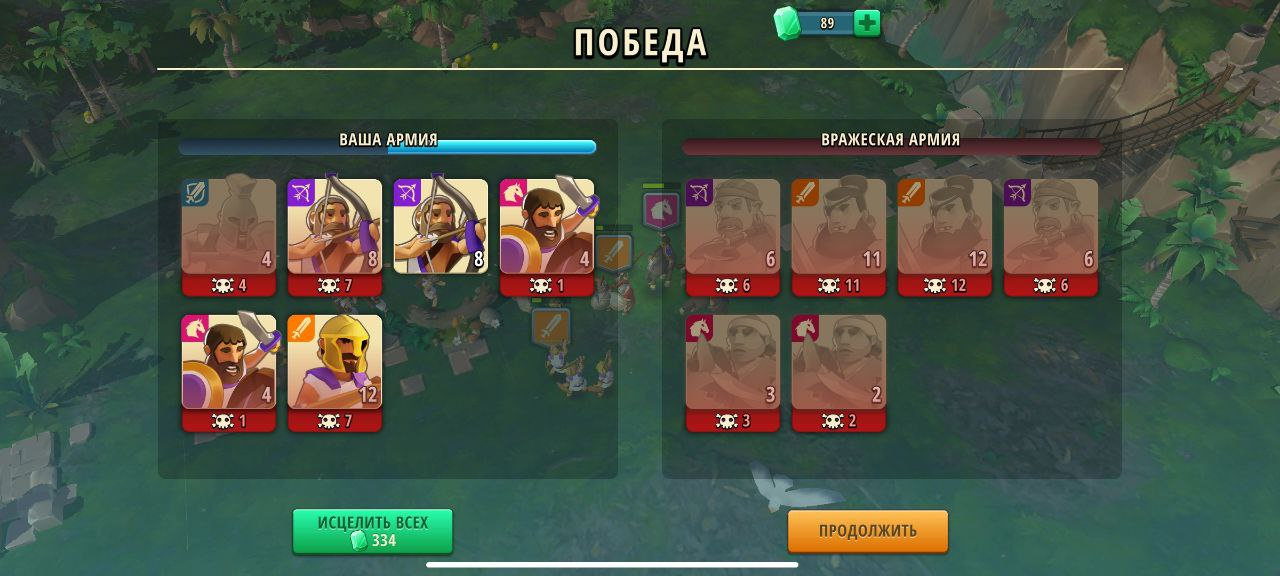
\includegraphics[width=0.75\linewidth]{./parts/media/TreasureHunt/26/decoder/photo_2022-04-06_18-11-23.jpg} \\
	\hline
	\multirow{6}{*}{27} & Preyton &
	\hypertarget{fight27}{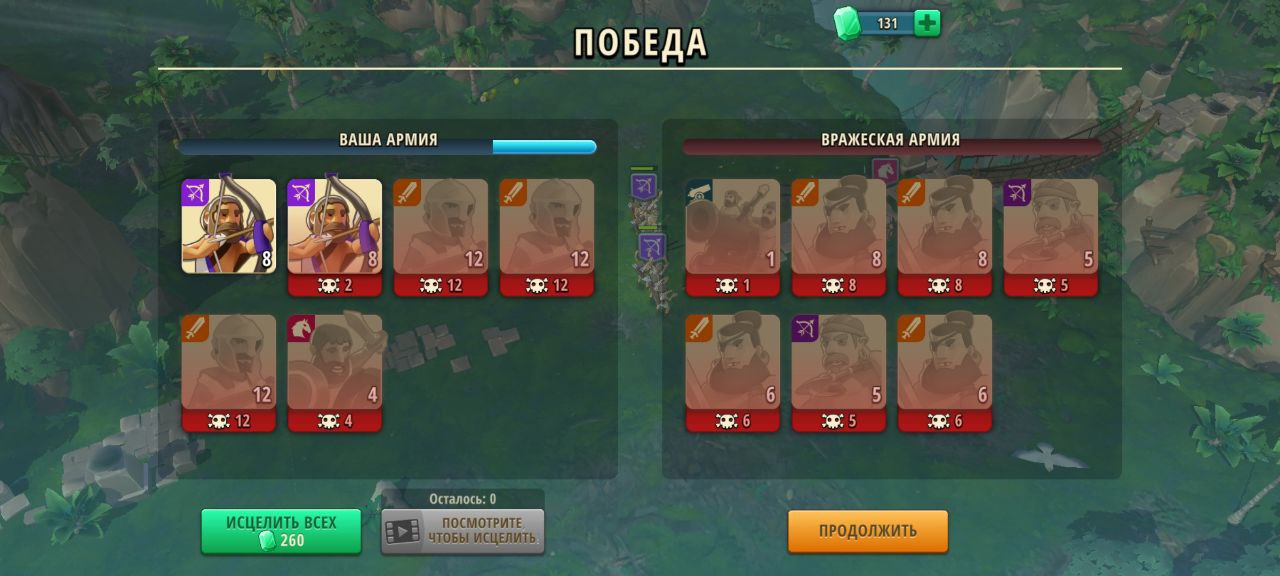
\includegraphics[width=0.75\linewidth]{./parts/media/TreasureHunt/27/Preyton/27..jpg}} \\
	& Preyton &
	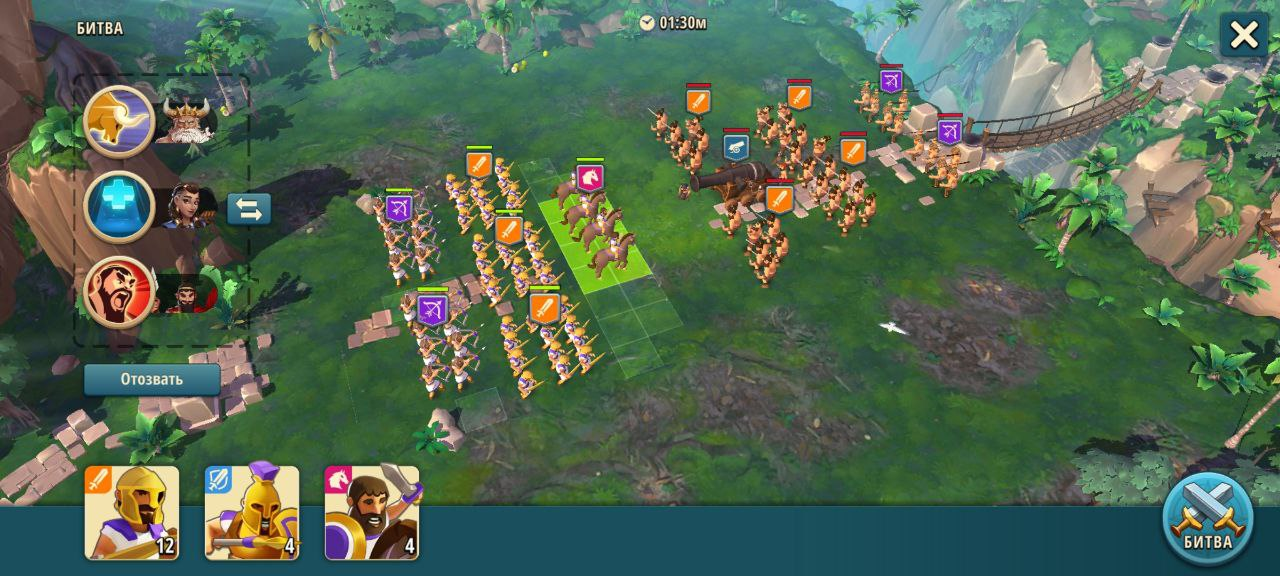
\includegraphics[width=0.75\linewidth]{./parts/media/TreasureHunt/27/Preyton/27.jpg} \\
	\hline
	\multirow{6}{*}{27} & Алексей &
	\hypertarget{fight27}{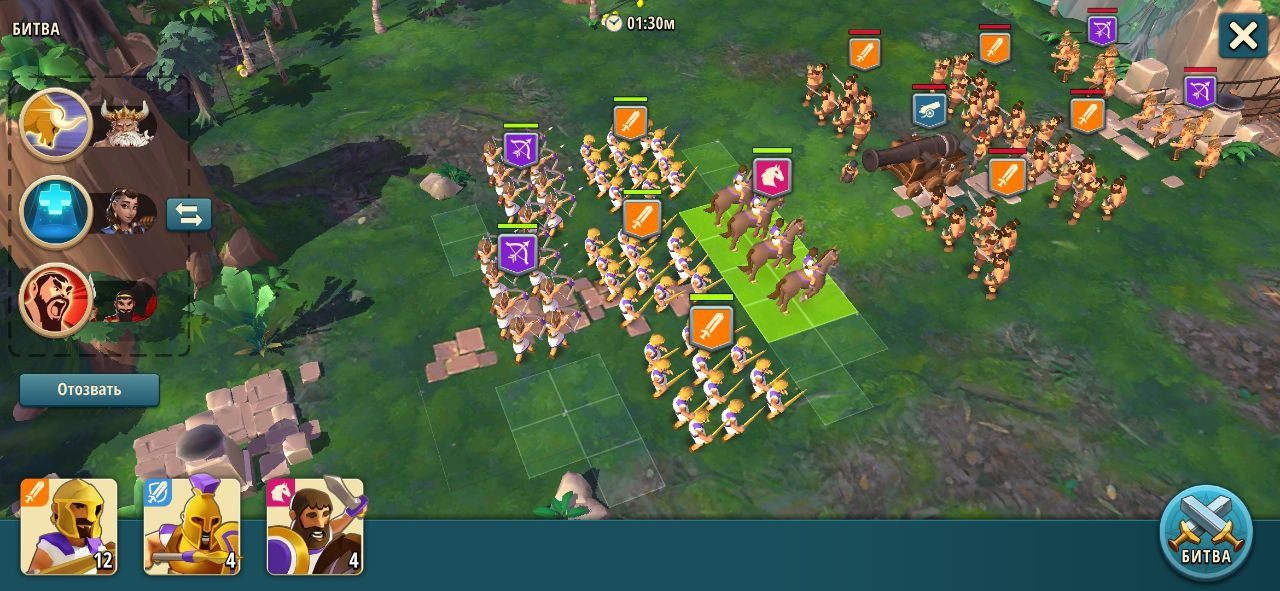
\includegraphics[width=0.75\linewidth]{./parts/media/TreasureHunt/27/alexey/photo_2022-04-14_12-34-58.jpg}} \\
	& Алексей &
	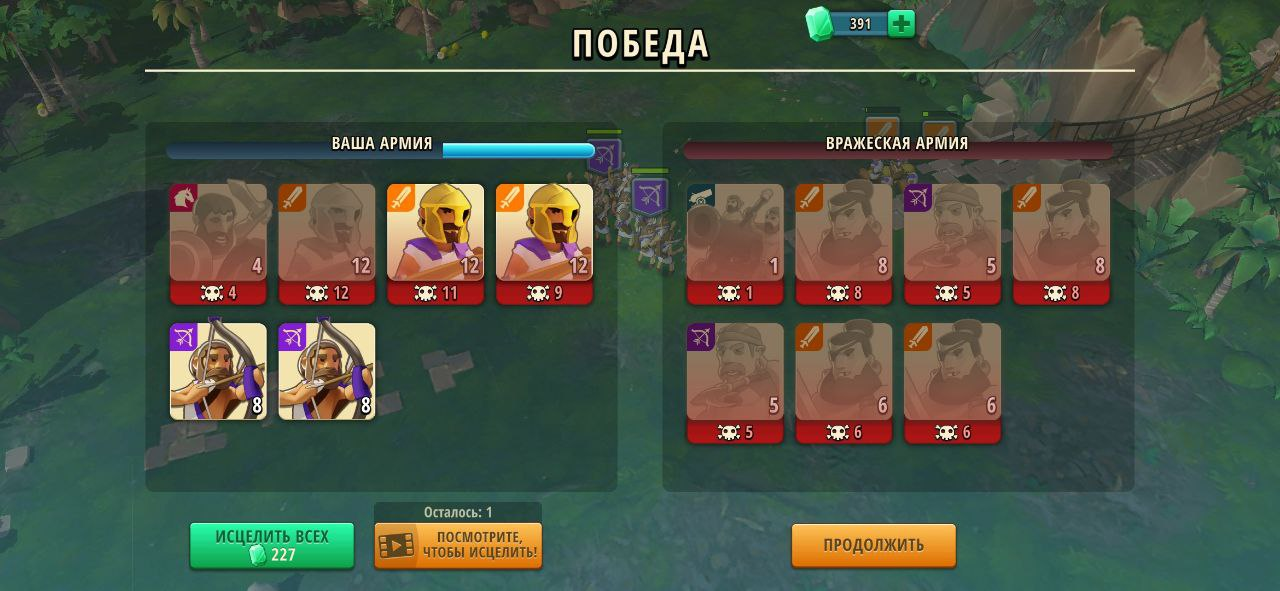
\includegraphics[width=0.75\linewidth]{./parts/media/TreasureHunt/27/alexey/photo_2022-04-14_12-34-36.jpg} \\
	\hline
	\multirow{6}{*}{27} & decoder &
	\hypertarget{fight27}{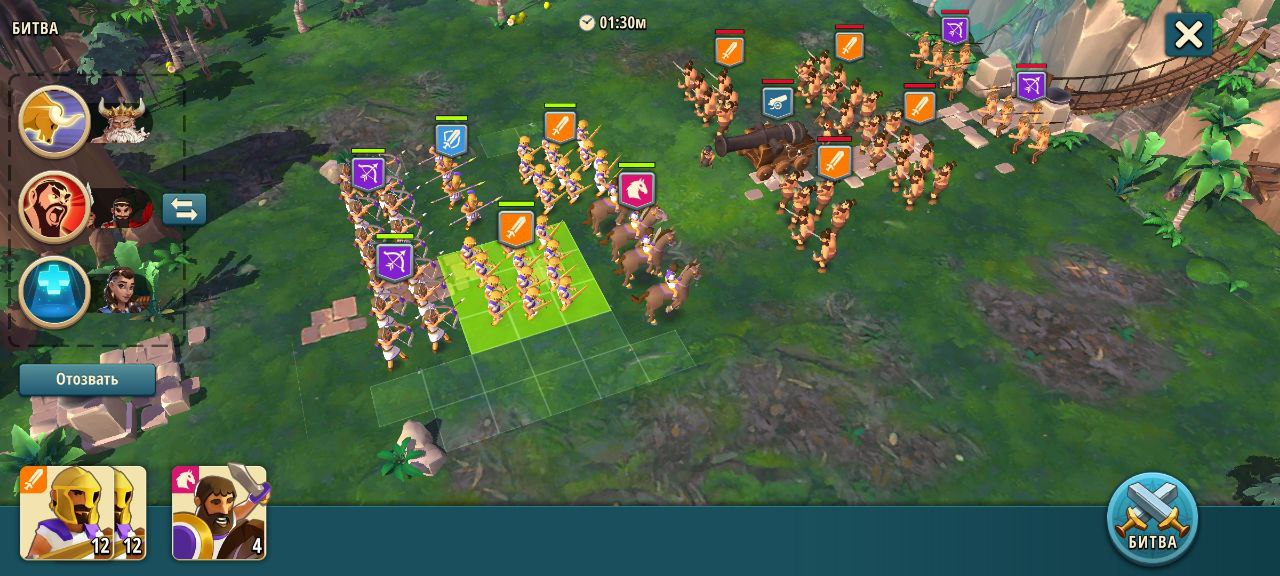
\includegraphics[width=0.75\linewidth]{./parts/media/TreasureHunt/27/decoder/photo_2022-04-13_17-26-43.jpg}} \\
	& decoder &
	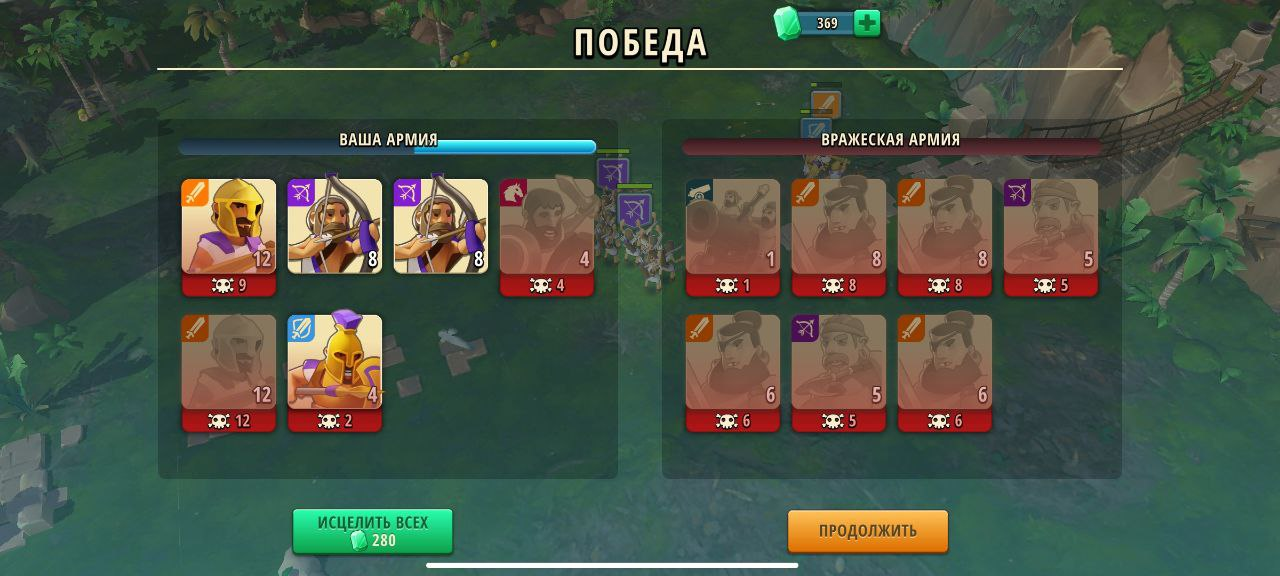
\includegraphics[width=0.75\linewidth]{./parts/media/TreasureHunt/27/decoder/photo_2022-04-13_17-27-02.jpg} \\
	\hline
	\multirow{4}{*}{28} & Preyton &
	\hypertarget{fight28}{\includegraphics[width=0.75\linewidth]{./parts/media/TreasureHunt/28/Preyton/28.jpg}} \\
	& Preyton &
	\includegraphics[width=0.75\linewidth]{./parts/media/TreasureHunt/28/Preyton/28..jpg} \\
	\hline
	\multirow{4}{*}{28} & decoder &
	\hypertarget{fight28}{\includegraphics[width=0.75\linewidth]{./parts/media/TreasureHunt/28/decoder/photo_2022-04-13_19-02-12.jpg}} \\
	& decoder &
	\includegraphics[width=0.75\linewidth]{./parts/media/TreasureHunt/28/decoder/photo_2022-04-13_19-02-29.jpg} \\
	\hline
	\multirow{8}{*}{29} & Sargon &
	\hypertarget{fight29}{\includegraphics[width=0.75\linewidth]{./parts/media/TreasureHunt/29/sargon/photo_2022-04-07_10-02-57.jpg}} \\
	& Sargon &
	\includegraphics[width=0.75\linewidth]{./parts/media/TreasureHunt/29/sargon/photo_2022-04-07_10-03-11.jpg} \\
	\hline
	\multirow{8}{*}{29} & Preyton &
	\hypertarget{fight29}{\includegraphics[width=0.75\linewidth]{./parts/media/TreasureHunt/29/Preyton/29.jpg}} \\
	& Preyton &
	\includegraphics[width=0.75\linewidth]{./parts/media/TreasureHunt/29/Preyton/29..jpg} \\
	\hline
	\multirow{8}{*}{29} & Алексей &
	\hypertarget{fight29}{\includegraphics[width=0.75\linewidth]{./parts/media/TreasureHunt/29/alexey/photo_2022-04-07_13-17-44.jpg}} \\
	& Алексей &
	\includegraphics[width=0.75\linewidth]{./parts/media/TreasureHunt/29/alexey/photo_2022-04-07_13-18-00.jpg} \\
	\hline
	\multirow{8}{*}{29} & decoder &
	\hypertarget{fight29}{\includegraphics[width=0.75\linewidth]{./parts/media/TreasureHunt/29/decoder/photo_2022-04-07_09-59-10.jpg}} \\
	& decoder &
	\includegraphics[width=0.75\linewidth]{./parts/media/TreasureHunt/29/decoder/photo_2022-04-07_09-59-23.jpg} \\
	\hline
	\multirow{15}{*}{30} & Sargon &
	\hypertarget{fight30}{\includegraphics[width=0.75\linewidth]{./parts/media/TreasureHunt/30/sargon/photo_2022-04-07_10-05-04.jpg}} \\
	& Sargon &
	\includegraphics[width=0.75\linewidth]{./parts/media/TreasureHunt/30/sargon/photo_2022-04-07_10-04-47.jpg} \\
	& Sargon &
	\includegraphics[width=0.75\linewidth]{./parts/media/TreasureHunt/30/sargon/photo_2022-04-07_10-05-00.jpg} \\
	\hline
	\multirow{15}{*}{30} & Preyton &
	\hypertarget{fight30}{\includegraphics[width=0.75\linewidth]{./parts/media/TreasureHunt/30/Preyton/30.2.jpg}} \\
	& Preyton &
	\includegraphics[width=0.75\linewidth]{./parts/media/TreasureHunt/30/Preyton/30.1.jpg} \\
	& Preyton &
	\includegraphics[width=0.75\linewidth]{./parts/media/TreasureHunt/30/Preyton/30_2.jpg} \\
	& Preyton &
	\includegraphics[width=0.75\linewidth]{./parts/media/TreasureHunt/30/Preyton/30_1.jpg} \\
	\hline
	\multirow{15}{*}{30} & Алексей &
	\hypertarget{fight30}{\includegraphics[width=0.75\linewidth]{./parts/media/TreasureHunt/30/alexey/photo_2022-04-14_12-36-02.jpg}} \\
	& Алексей &
	\includegraphics[width=0.75\linewidth]{./parts/media/TreasureHunt/30/alexey/photo_2022-04-14_12-35-50.jpg} \\
	& Алексей &
	\includegraphics[width=0.75\linewidth]{./parts/media/TreasureHunt/30/alexey/photo_2022-04-14_12-36-06.jpg} \\
	& Алексей &
	\includegraphics[width=0.75\linewidth]{./parts/media/TreasureHunt/30/alexey/photo_2022-04-14_12-35-59.jpg} \\
	\hline
	\multirow{15}{*}{30} & decoder &
	\hypertarget{fight30}{\includegraphics[width=0.75\linewidth]{./parts/media/TreasureHunt/30/decoder/photo_2022-04-07_10-00-32.jpg}} \\
	& decoder &
	\includegraphics[width=0.75\linewidth]{./parts/media/TreasureHunt/30/decoder/photo_2022-04-07_09-59-28.jpg} \\
	& decoder &
	\includegraphics[width=0.75\linewidth]{./parts/media/TreasureHunt/30/decoder/photo_2022-04-07_09-59-40.jpg} \\
	& decoder &
	\includegraphics[width=0.75\linewidth]{./parts/media/TreasureHunt/30/decoder/photo_2022-04-07_10-00-22.jpg} \\
	\hline
	\multirow{12}{*}{31} & Sargon &
	\hypertarget{fight31}{\includegraphics[width=0.75\linewidth]{./parts/media/TreasureHunt/31/sargon/photo_2022-04-07_10-05-18.jpg}} \\
	& Sargon &
	\includegraphics[width=0.75\linewidth]{./parts/media/TreasureHunt/31/sargon/photo_2022-04-07_10-05-22.jpg} \\
	& Sargon &
	\includegraphics[width=0.75\linewidth]{./parts/media/TreasureHunt/31/sargon/photo_2022-04-07_10-05-08.jpg} \\
	& Sargon &
	\includegraphics[width=0.75\linewidth]{./parts/media/TreasureHunt/31/sargon/photo_2022-04-07_10-05-25.jpg} \\
	\hline
	\multirow{12}{*}{31} & Preyton &
	\hypertarget{fight31}{\includegraphics[width=0.75\linewidth]{./parts/media/TreasureHunt/31/Preyton/31_2.jpg}} \\
	& Preyton &
	\includegraphics[width=0.75\linewidth]{./parts/media/TreasureHunt/31/Preyton/31_1.jpg} \\
	& Preyton &
	\includegraphics[width=0.75\linewidth]{./parts/media/TreasureHunt/31/Preyton/31.2.jpg} \\
	& Preyton &
	\includegraphics[width=0.75\linewidth]{./parts/media/TreasureHunt/31/Preyton/31.1.jpg} \\
	\hline
	\multirow{12}{*}{31} & decoder &
	\hypertarget{fight31}{\includegraphics[width=0.75\linewidth]{./parts/media/TreasureHunt/31/decoder/photo_2022-04-07_09-59-48.jpg}} \\
	& decoder &
	\includegraphics[width=0.75\linewidth]{./parts/media/TreasureHunt/31/decoder/photo_2022-04-07_09-59-58.jpg} \\
	& decoder &
	\includegraphics[width=0.75\linewidth]{./parts/media/TreasureHunt/31/decoder/photo_2022-04-07_10-00-36.jpg} \\
	& decoder &
	\includegraphics[width=0.75\linewidth]{./parts/media/TreasureHunt/31/decoder/photo_2022-04-07_10-00-46.jpg} \\
	\hline
	\multirow{16}{*}{32} & Sargon &
	\hypertarget{fight32}{\includegraphics[width=0.75\linewidth]{./parts/media/TreasureHunt/32/sargon/photo_2022-04-07_10-05-45.jpg}} \\
	& Sargon &
	\includegraphics[width=0.75\linewidth]{./parts/media/TreasureHunt/32/sargon/photo_2022-04-07_10-05-39.jpg} \\
	& Sargon &
	\includegraphics[width=0.75\linewidth]{./parts/media/TreasureHunt/32/sargon/photo_2022-04-07_10-05-31.jpg} \\
	& Sargon &
	\includegraphics[width=0.75\linewidth]{./parts/media/TreasureHunt/32/sargon/photo_2022-04-07_10-05-42.jpg} \\
	\hline
	\multirow{16}{*}{32} & Preyton &
	\hypertarget{fight32}{\includegraphics[width=0.75\linewidth]{./parts/media/TreasureHunt/32/Preyton/32.2.jpg}} \\
	& Preyton &
	\includegraphics[width=0.75\linewidth]{./parts/media/TreasureHunt/32/Preyton/32_2.jpg} \\
	& Preyton &
	\includegraphics[width=0.75\linewidth]{./parts/media/TreasureHunt/32/Preyton/32_1.jpg} \\
	& Preyton &
	\includegraphics[width=0.75\linewidth]{./parts/media/TreasureHunt/32/Preyton/32.1.jpg} \\
	\hline
	\multirow{16}{*}{32} & Алексей &
	\hypertarget{fight32}{\includegraphics[width=0.75\linewidth]{./parts/media/TreasureHunt/32/alexey/photo_2022-04-14_13-54-49.jpg}} \\
	& Алексей &
	\includegraphics[width=0.75\linewidth]{./parts/media/TreasureHunt/32/alexey/photo_2022-04-14_13-54-23.jpg} \\
	& Алексей &
	\includegraphics[width=0.75\linewidth]{./parts/media/TreasureHunt/32/alexey/photo_2022-04-14_13-54-53.jpg} \\
	& Алексей &
	\includegraphics[width=0.75\linewidth]{./parts/media/TreasureHunt/32/alexey/photo_2022-04-14_13-54-58.jpg} \\
	\hline
	\multirow{16}{*}{32} & decoder &
	\hypertarget{fight32}{\includegraphics[width=0.75\linewidth]{./parts/media/TreasureHunt/32/decoder/photo_2022-04-07_10-00-59.jpg}} \\
	& decoder &
	\includegraphics[width=0.75\linewidth]{./parts/media/TreasureHunt/32/decoder/photo_2022-04-07_10-01-57.jpg} \\
	& decoder &
	\includegraphics[width=0.75\linewidth]{./parts/media/TreasureHunt/32/decoder/photo_2022-04-07_10-01-54.jpg} \\
	& decoder &
	\includegraphics[width=0.75\linewidth]{./parts/media/TreasureHunt/32/decoder/photo_2022-04-07_10-01-48.jpg} \\
	\hline
	\multirow{12}{*}{33} & Sargon &
	\hypertarget{fight33}{\includegraphics[width=0.75\linewidth]{./parts/media/TreasureHunt/33/sargon/photo_2022-04-07_10-06-40.jpg}} \\
	& Sargon &
	\includegraphics[width=0.75\linewidth]{./parts/media/TreasureHunt/33/sargon/photo_2022-04-07_10-06-37.jpg} \\
	& Sargon &
	\includegraphics[width=0.75\linewidth]{./parts/media/TreasureHunt/33/sargon/photo_2022-04-07_10-06-22.jpg} \\
	& Sargon &
	\includegraphics[width=0.75\linewidth]{./parts/media/TreasureHunt/33/sargon/photo_2022-04-07_10-06-34.jpg} \\
	\hline
	\multirow{12}{*}{33} & Preyton &
	\hypertarget{fight33}{\includegraphics[width=0.75\linewidth]{./parts/media/TreasureHunt/33/Preyton/33_1.jpg}} \\
	& Preyton &
	\includegraphics[width=0.75\linewidth]{./parts/media/TreasureHunt/33/Preyton/33_2.jpg} \\
	& Preyton &
	\includegraphics[width=0.75\linewidth]{./parts/media/TreasureHunt/33/Preyton/33.2.jpg} \\
	& Preyton &
	\includegraphics[width=0.75\linewidth]{./parts/media/TreasureHunt/33/Preyton/33.1.jpg} \\
	\hline
	\multirow{12}{*}{33} & decoder &
	\hypertarget{fight33}{\includegraphics[width=0.75\linewidth]{./parts/media/TreasureHunt/33/decoder/photo_2022-04-07_10-02-11.jpg}} \\
	& decoder &
	\includegraphics[width=0.75\linewidth]{./parts/media/TreasureHunt/33/decoder/photo_2022-04-07_10-02-27.jpg} \\
	& decoder &
	\includegraphics[width=0.75\linewidth]{./parts/media/TreasureHunt/33/decoder/photo_2022-04-07_10-02-23.jpg} \\
	& decoder &
	\includegraphics[width=0.75\linewidth]{./parts/media/TreasureHunt/33/decoder/photo_2022-04-07_10-02-19.jpg} \\
	\hline
	\multirow{12}{*}{34} & Sargon &
	\hypertarget{fight34}{\includegraphics[width=0.75\linewidth]{./parts/media/TreasureHunt/34/sargon/photo_2022-04-07_10-08-16.jpg}} \\
	& Sargon &
	\includegraphics[width=0.75\linewidth]{./parts/media/TreasureHunt/34/sargon/photo_2022-04-07_10-08-23.jpg} \\
	& Sargon &
	\includegraphics[width=0.75\linewidth]{./parts/media/TreasureHunt/34/sargon/photo_2022-04-07_10-08-04.jpg} \\
	& Sargon &
	\includegraphics[width=0.75\linewidth]{./parts/media/TreasureHunt/34/sargon/photo_2022-04-07_10-08-19.jpg} \\
	\hline
	\multirow{12}{*}{34} & Preyton &
	\hypertarget{fight34}{\includegraphics[width=0.75\linewidth]{./parts/media/TreasureHunt/34/Preyton/34_2.jpg}} \\
	& Preyton &
	\includegraphics[width=0.75\linewidth]{./parts/media/TreasureHunt/34/Preyton/34.1.jpg} \\
	& Preyton &
	\includegraphics[width=0.75\linewidth]{./parts/media/TreasureHunt/34/Preyton/34_1.jpg} \\
	& Preyton &
	\includegraphics[width=0.75\linewidth]{./parts/media/TreasureHunt/34/Preyton/34.2.jpg} \\
	\hline
	\multirow{12}{*}{34} & decoder &
	\hypertarget{fight34}{\includegraphics[width=0.75\linewidth]{./parts/media/TreasureHunt/34/decoder/photo_2022-04-07_10-02-46.jpg}} \\
	& decoder &
	\includegraphics[width=0.75\linewidth]{./parts/media/TreasureHunt/34/decoder/photo_2022-04-07_10-02-50.jpg} \\
	& decoder &
	\includegraphics[width=0.75\linewidth]{./parts/media/TreasureHunt/34/decoder/photo_2022-04-07_10-02-43.jpg} \\
	& decoder &
	\includegraphics[width=0.75\linewidth]{./parts/media/TreasureHunt/34/decoder/photo_2022-04-07_10-02-34.jpg} \\
	\hline
	\multirow{12}{*}{35} & Sargon &
	\hypertarget{fight35}{\includegraphics[width=0.75\linewidth]{./parts/media/TreasureHunt/35/sargon/photo_2022-04-07_10-08-45.jpg}} \\
	& Sargon &
	\includegraphics[width=0.75\linewidth]{./parts/media/TreasureHunt/35/sargon/photo_2022-04-07_10-08-41.jpg} \\
	& Sargon &
	\includegraphics[width=0.75\linewidth]{./parts/media/TreasureHunt/35/sargon/photo_2022-04-07_10-08-48.jpg} \\
	& Sargon &
	\includegraphics[width=0.75\linewidth]{./parts/media/TreasureHunt/35/sargon/photo_2022-04-07_10-08-33.jpg} \\
	\hline
	\multirow{12}{*}{35} & Preyton &
	\hypertarget{fight35}{\includegraphics[width=0.75\linewidth]{./parts/media/TreasureHunt/35/Preyton/35_1.jpg}} \\
	& Preyton &
	\includegraphics[width=0.75\linewidth]{./parts/media/TreasureHunt/35/Preyton/35.2.jpg} \\
	& Preyton &
	\includegraphics[width=0.75\linewidth]{./parts/media/TreasureHunt/35/Preyton/35_2.jpg} \\
	& Preyton &
	\includegraphics[width=0.75\linewidth]{./parts/media/TreasureHunt/35/Preyton/35.1.jpg} \\
	\hline
	\multirow{12}{*}{35} & decoder &
	\hypertarget{fight35}{\includegraphics[width=0.75\linewidth]{./parts/media/TreasureHunt/35/decoder/photo_2022-04-07_10-05-55.jpg}} \\
	& decoder &
	\includegraphics[width=0.75\linewidth]{./parts/media/TreasureHunt/35/decoder/photo_2022-04-07_10-06-14.jpg} \\
	& decoder &
	\includegraphics[width=0.75\linewidth]{./parts/media/TreasureHunt/35/decoder/photo_2022-04-07_10-06-11.jpg} \\
	& decoder &
	\includegraphics[width=0.75\linewidth]{./parts/media/TreasureHunt/35/decoder/photo_2022-04-07_10-06-08.jpg} \\
	\hline
	\multirow{16}{*}{36} & Sargon &
	\hypertarget{fight36}{\includegraphics[width=0.75\linewidth]{./parts/media/TreasureHunt/36/sargon/photo_2022-04-07_13-16-23.jpg}} \\
	& Sargon &
	\includegraphics[width=0.75\linewidth]{./parts/media/TreasureHunt/36/sargon/photo_2022-04-07_13-16-46.jpg} \\
	& Sargon &
	\includegraphics[width=0.75\linewidth]{./parts/media/TreasureHunt/36/sargon/photo_2022-04-07_13-16-43.jpg} \\
	& Sargon &
	\includegraphics[width=0.75\linewidth]{./parts/media/TreasureHunt/36/sargon/photo_2022-04-07_13-16-40.jpg} \\
	\hline
	\multirow{16}{*}{36} & Preyton &
	\hypertarget{fight36}{\includegraphics[width=0.75\linewidth]{./parts/media/TreasureHunt/36/Preyton/36_2.jpg}} \\
	& Preyton &
	\includegraphics[width=0.75\linewidth]{./parts/media/TreasureHunt/36/Preyton/36_1.jpg} \\
	& Preyton &
	\includegraphics[width=0.75\linewidth]{./parts/media/TreasureHunt/36/Preyton/36.1.jpg} \\
	& Preyton &
	\includegraphics[width=0.75\linewidth]{./parts/media/TreasureHunt/36/Preyton/36.2.jpg} \\
	\hline
	\multirow{16}{*}{36} & Алексей &
	\hypertarget{fight36}{\includegraphics[width=0.75\linewidth]{./parts/media/TreasureHunt/36/alexey/photo_2022-04-15_11-02-44.jpg}} \\
	& Алексей &
	\includegraphics[width=0.75\linewidth]{./parts/media/TreasureHunt/36/alexey/photo_2022-04-15_11-02-55.jpg} \\
	& Алексей &
	\includegraphics[width=0.75\linewidth]{./parts/media/TreasureHunt/36/alexey/photo_2022-04-15_11-02-05.jpg} \\
	& Алексей &
	\includegraphics[width=0.75\linewidth]{./parts/media/TreasureHunt/36/alexey/photo_2022-04-15_11-02-50.jpg} \\
	\hline
	\multirow{16}{*}{36} & decoder &
	\hypertarget{fight36}{\includegraphics[width=0.75\linewidth]{./parts/media/TreasureHunt/36/decoder/photo_2022-04-07_10-07-36.jpg}} \\
	& decoder &
	\includegraphics[width=0.75\linewidth]{./parts/media/TreasureHunt/36/decoder/photo_2022-04-07_10-07-28.jpg} \\
	& decoder &
	\includegraphics[width=0.75\linewidth]{./parts/media/TreasureHunt/36/decoder/photo_2022-04-07_10-07-32.jpg} \\
	& decoder &
	\includegraphics[width=0.75\linewidth]{./parts/media/TreasureHunt/36/decoder/photo_2022-04-07_10-07-13.jpg} \\
	\hline
	\multirow{12}{*}{37} & Sargon &
	\hypertarget{fight37}{\includegraphics[width=0.75\linewidth]{./parts/media/TreasureHunt/37/sargon/photo_2022-04-07_13-17-09.jpg}} \\
	& Sargon &
	\includegraphics[width=0.75\linewidth]{./parts/media/TreasureHunt/37/sargon/photo_2022-04-07_13-16-57.jpg} \\
	& Sargon &
	\includegraphics[width=0.75\linewidth]{./parts/media/TreasureHunt/37/sargon/photo_2022-04-07_13-17-01.jpg} \\
	& Sargon &
	\includegraphics[width=0.75\linewidth]{./parts/media/TreasureHunt/37/sargon/photo_2022-04-07_13-16-49.jpg} \\
	\hline
	\multirow{12}{*}{37} & Preyton &
	\hypertarget{fight37}{\includegraphics[width=0.75\linewidth]{./parts/media/TreasureHunt/37/Preyton/37_1.jpg}} \\
	& Preyton &
	\includegraphics[width=0.75\linewidth]{./parts/media/TreasureHunt/37/Preyton/37_2.jpg} \\
	& Preyton &
	\includegraphics[width=0.75\linewidth]{./parts/media/TreasureHunt/37/Preyton/37.2.jpg} \\
	& Preyton &
	\includegraphics[width=0.75\linewidth]{./parts/media/TreasureHunt/37/Preyton/37.1.jpg} \\
	\hline
	\multirow{12}{*}{37} & decoder &
	\hypertarget{fight37}{\includegraphics[width=0.75\linewidth]{./parts/media/TreasureHunt/37/decoder/photo_2022-04-14_12-36-24.jpg}} \\
	& decoder &
	\includegraphics[width=0.75\linewidth]{./parts/media/TreasureHunt/37/decoder/photo_2022-04-14_12-36-38.jpg} \\
	& decoder &
	\includegraphics[width=0.75\linewidth]{./parts/media/TreasureHunt/37/decoder/photo_2022-04-14_12-36-42.jpg} \\
	& decoder &
	\includegraphics[width=0.75\linewidth]{./parts/media/TreasureHunt/37/decoder/photo_2022-04-14_12-36-46.jpg} \\
	\hline
	\multirow{12}{*}{38} & Sargon &
	\hypertarget{fight38}{\includegraphics[width=0.75\linewidth]{./parts/media/TreasureHunt/38/sargon/photo_2022-04-07_13-17-35.jpg}} \\
	& Sargon &
	\includegraphics[width=0.75\linewidth]{./parts/media/TreasureHunt/38/sargon/photo_2022-04-07_13-17-20.jpg} \\
	& Sargon &
	\includegraphics[width=0.75\linewidth]{./parts/media/TreasureHunt/38/sargon/photo_2022-04-07_13-17-28.jpg} \\
	& Sargon &
	\includegraphics[width=0.75\linewidth]{./parts/media/TreasureHunt/38/sargon/photo_2022-04-07_13-17-31.jpg} \\
	\hline
	\multirow{12}{*}{38} & Preyton &
	\hypertarget{fight38}{\includegraphics[width=0.75\linewidth]{./parts/media/TreasureHunt/38/Preyton/38_2.jpg}} \\
	& Preyton &
	\includegraphics[width=0.75\linewidth]{./parts/media/TreasureHunt/38/Preyton/38.1.jpg} \\
	& Preyton &
	\includegraphics[width=0.75\linewidth]{./parts/media/TreasureHunt/38/Preyton/38_1.jpg} \\
	& Preyton &
	\includegraphics[width=0.75\linewidth]{./parts/media/TreasureHunt/38/Preyton/38.2.jpg} \\
	\hline
	\multirow{12}{*}{38} & decoder &
	\hypertarget{fight38}{\includegraphics[width=0.75\linewidth]{./parts/media/TreasureHunt/38/decoder/photo_2022-04-07_10-10-23.jpg}} \\
	& decoder &
	\includegraphics[width=0.75\linewidth]{./parts/media/TreasureHunt/38/decoder/photo_2022-04-07_10-10-16.jpg} \\
	& decoder &
	\includegraphics[width=0.75\linewidth]{./parts/media/TreasureHunt/38/decoder/photo_2022-04-07_10-10-01.jpg} \\
	& decoder &
	\includegraphics[width=0.75\linewidth]{./parts/media/TreasureHunt/38/decoder/photo_2022-04-07_10-10-19.jpg} \\
	\hline
	\multirow{11}{*}{39} & Sargon &
	\hypertarget{fight39}{\includegraphics[width=0.75\linewidth]{./parts/media/TreasureHunt/39/sargon/photo_2022-04-07_13-18-09.jpg}} \\
	& Sargon &
	\includegraphics[width=0.75\linewidth]{./parts/media/TreasureHunt/39/sargon/photo_2022-04-07_13-18-26.jpg} \\
	& Sargon &
	\includegraphics[width=0.75\linewidth]{./parts/media/TreasureHunt/39/sargon/photo_2022-04-07_13-18-21.jpg} \\
	& Sargon &
	\includegraphics[width=0.75\linewidth]{./parts/media/TreasureHunt/39/sargon/photo_2022-04-07_13-18-31.jpg} \\
	\hline
	\multirow{11}{*}{39} & Preyton &
	\hypertarget{fight39}{\includegraphics[width=0.75\linewidth]{./parts/media/TreasureHunt/39/Preyton/39_1.jpg}} \\
	& Preyton &
	\includegraphics[width=0.75\linewidth]{./parts/media/TreasureHunt/39/Preyton/39.2.jpg} \\
	& Preyton &
	\includegraphics[width=0.75\linewidth]{./parts/media/TreasureHunt/39/Preyton/39.1.jpg} \\
	\hline
	\multirow{11}{*}{39} & decoder &
	\hypertarget{fight39}{\includegraphics[width=0.75\linewidth]{./parts/media/TreasureHunt/39/decoder/photo_2022-04-07_13-15-36.jpg}} \\
	& decoder &
	\includegraphics[width=0.75\linewidth]{./parts/media/TreasureHunt/39/decoder/photo_2022-04-07_13-15-27.jpg} \\
	& decoder &
	\includegraphics[width=0.75\linewidth]{./parts/media/TreasureHunt/39/decoder/photo_2022-04-07_13-15-43.jpg} \\
	& decoder &
	\includegraphics[width=0.75\linewidth]{./parts/media/TreasureHunt/39/decoder/photo_2022-04-07_13-15-39.jpg} \\
	\hline
	\multirow{4}{*}{40} & decoder &
	\hypertarget{fight40}{\includegraphics[width=0.75\linewidth]{./parts/media/TreasureHunt/40/decoder/photo_2022-04-07_13-16-08.jpg}} \\
	& decoder &
	\includegraphics[width=0.75\linewidth]{./parts/media/TreasureHunt/40/decoder/photo_2022-04-07_13-16-15.jpg} \\
	& decoder &
	\includegraphics[width=0.75\linewidth]{./parts/media/TreasureHunt/40/decoder/photo_2022-04-07_13-16-12.jpg} \\
	& decoder &
	\includegraphics[width=0.75\linewidth]{./parts/media/TreasureHunt/40/decoder/photo_2022-04-07_13-15-51.jpg} \\
	\hline
\end{longtable}

    \section{Охота за Сокровищами} 

\subsection{Прохождение боями во время перехода между эпохами}
\label{subsection:treasure_between_epochs}

Делать так можно не часто, но призы в конце стоят того. 
Перед переходом в следующую эпоху затормозите на некоторое время (подробнее в \ref{section:epochs}). 
Копите ресурсы, торгуйте, проходите сокровища в обычном темпе. 
Колбы сливайте в Чудеса членов нашего Альянса.
И не открывайте сундуки! Их вы откроете (постепенно), когда перейдёте в новую эпоху. 
Главное -- набрать достаточное количество ресурсов, чтобы в новой эпохе разом (за день) прокачать хотя бы 2 рода войск. 
Также имеет смысл проходить компанию до упора: новые командиры -- это ваше решающее преимущество.

Когда вы накопите достаточно ресурсов, ждите начала новых сокровищ. 
И сразу, как начнёте их проходить, переходите в новую эпоху.
Дело в том, что сложность боёв выставляется в начале Сокровищ.
Так вы сможете без единого самоцвета и переговоров легко пройти все 60 боёв.

\subsection{Прохождение боями с накоплением улучшений}

Первые два уровня легко проходятся без всяких усилений.
Возможно последние 5 битв придётся проходить переговорами.
Но они довольно лёгкие.

А теперь представим себе ситуацию: Вы копите улучшения и не ставите их
довольно продолжительное время. Больше всего можно поставить домов с
черепушкой.

Дома черепушки попадаются в двух сундуках-чек-поинтах, которые мы всегда берём (с вероятностями 10\% и 20\%),
а также на боях с номерами 30, 39, 40, 44, 54 и 60 (с вероятностью 20\% на каждом).
Бои 54 и 60 можно сразу отбросить. До них сложно дойти. Если есть возможность -- отлично!
Но, если доходить до 44, в среднем за неделю выпадает 1.1 дом с черепушкой.
За это же время выпадает 0.9 улучшений конницы,
0.5 улучшений тяжёлой пехоты,
0.6 улучшений артиллерии (которую в Греции некуда девать),
0.8 улучшений луков.
Но важны по сути только дома с черепушкой. Их в конце Греции 18 (и каждый даёт по 5\% усиления пехоте).
Значить собирать их всех придётся примерно 4.1 месяца.

Это конечно даст 90\% усиления пехоте в Греции, но этого и не нужно.
От Минойской эры до Греции пехота усиливается приблизительно на 15\%. 
От Греции до Древнего Рима -- примерно на 20\%. Это значит, что 6 домов с черепами (30\% усиления пехоты) должно хватать для простого прохождения Сокровищ только боями. 
А это примерно 5.5 недель (предполагается, что Зевс даёт хотя бы 10\%).
Уже более реальная цифра, чем 4 месяца.

Но для более плавного и спокойного прохождения лучше подождать 8 домов-черепушек.
Дело в том, что максимальное улучшение на пиратах — 40\%.
При переходе к новой эпохе у войск растёт не только атака, но и жизнеспособность.
Поэтому нужно компенсировать жизнеспособность атакой.
Однако разницу в 10\% должно быть возможно возместить наличием у нас Командиров-способностей.

В конце Греции на малых и средних объектах культуры можно разместить:
\begin{itemize}
    \item 20\% на коней или тяжёлую пехоту,
    \item 35\% на артиллерию или луки.
\end{itemize}
Строго необходимо разместить все 20\% на коней и 35\% на луки.
При этом ничего не мешает ставить в любое время улучшения тяжёлой пехоты и артиллерии.
Кроме того во время ивента так же можно экономить улучшения войск.

В итоге.
Рецепт должен быть такими.
Примерно 5 недель (пока не накопится 6 домов с черепашками) не ставить ни одного улучшения армии. Потом поставить всё в начале 3 уровня Сокровищ. Должно хватить на 2 полных прохождения Сокровищ.


\subsection{Переговоры}

Начальные переговоры на 3 товара удобнее всего проходить следующим образом. 
На первом этапе всем предлагаем монеты. 
На втором -- еду. 
На третьем -- товар.
Проиграть нельзя.

Далее о более сложных переговорах.

На первом этапе нужно выставить все разные товары. 
Если товаров меньше, чем пиратов, можно выставить несколько единиц самого дешёвого товара (обычно это монеты: имеется ввиду субъективная ценность для Вас в текущей ситуации (то чего мало -- дорого)). 
Если товаров больше, чем пиратов, начинать нужно с выставления самых дешёвых товаров.

Цель первых двух этапов определить, что не нужно ни кому.

На втором этапе продолжайте выставлять в первую очередь те товары, которые ещё не выставляли. 
Во вторую те, которые ещё ни кто не принял. 
Далее опять-таки самый дешёвый товар.

На третьем этапе некоторые пираты уже приняли товар, а для некоторых становится возможно однозначно определить их выбор по тому, что они отвергли. 
Их выставляйте в первую очередь и приравнивание к уже принявшим. 
Затем нужно посчитать какие товары из оставшихся пока не были приняты, какие были приняты единожды, дважды... 
Таким образом получается частота принятия $\nu_i \geqslant 0$ товара с номером $i$.
Очевидно, что чем больше на данный момент частота принятия некоторого товара, тем меньше вероятность того, что он ещё кому-то нужен. 
Так и выставляйте: от наименьшей частоты  к наибольшей.
Если $\nu_{i_1} \leqslant \nu_{i_2} \leqslant \ldots \leqslant \nu_{i_k}$, то выставлять товары в очерёдности $i_1, i_2, \ldots, i_k$. 

То есть, на пример, сначала находим пирата, которому ещё можно предложить товар, который ещё ни кем не принят (частота принятия $\nu_{i_1} = 0$). Предлагаем и засчитываем товару частоту принятия $\nu_{i_1} = 1$. Для следующего пирата (предположим) уже нет товаров с частотой принятия 0. Тогда выбираем для него товар с частотой $\nu_{i_2} = 1$ и присваиваем данному товару частоту $\nu_{i_2} = 2$\ldots

Обязательно следите за тем, что говорят вам пираты о товарах, которые нужны другим пиратам.
Не обращайте внимания на то, что они отвечают последовательно.
Если на третьем этапе у вас осталось 5 возможных товаров, но вы угадали, что нужно всем кроме двух пиратов, а эти пираты говорят, что товар нужен другому пирату, значит, не смотря на то, что, например, этот товар именно сейчас подошёл пятому пирату, который ответил последним, имеется ввиду, что он нужен именно тому, кого вы не угадали.
Просто поменяйте товары местами и вы выиграли.
Так же можно размышлять и для 3 товаров, но уже с некоторой вероятностью неуспеха.

Теперь самое интересное -- переговоры с колбами. 
Не начинайте переговоры без колб, но не спешите их отдавать. 
Первые два этапа переговоров считайте, что колбы ни кому не нужны. 
И только на третьем этапе в случае, если становится однозначно известно, что какому-то пирату нужна именно колба, давайте её ему.

\subsection{Сундуки-чек-поинты}

Самые вкусные награды лежат в сундуках-чек-поинтах. Все 12 мы брать не сможем. 
Для этого все 20 членов должны пройти по 60 битв. Это фантастика. 
Но мы можем более или менее стабильно брать по 9 сундуков. 
Для этого нам нужно собираться пачками по 5-6 человек, которые готовы пройти все 60 битв по одной из представленных выше стратегий.

Уже в 9-ом сундуке с 35\%-ной вероятностью лежат 2 жетона Пиратской Крепости.

Можно искуственно увеличивать себе количество попыток в Охоте за Сокровищами один раз в две недели.
Для этого одну неделю нужно вообще не брать сундуков-чек-поинтов.
И не брать их даже после конца текущей Охоты.
Открывать их нужно после 16:00.
В это время, положенные Вам стартовые 4 попытки сами регенерируются.
После открытия сундуков можно получить ещё 20 попыток и начать следующую охоту с 24-мя попытками!
Это позволит легко пройти первый уровень в первый день.

Лучше всего синхронизировать недели с товарищами по Альянсу.
Так мы сможем очень быстро открывать третий уровень.

Сразу скажу, что во время тестирования данной стратегии я прошёл 59 битв, не открывая сундуков.

    \section{Ивенты}

Довольно важный вопрос: какие сундуки (амфоры, \ldots) открывать?
Рассмотрим ситуацию на примере ивента <<Кельты 2022 г.>>.
Все большие ивенты в игре имеют одинаковую механику, так что в дальнейшем стратегия их прохождения не поменяется.

Всего примерно 76500 очков. 
Возьмём среднюю стоимость сундуком по 265, 590 и 765.
В любых ивентах это будет соответствовать маленькому, среднему и большому сундукам.

Если считать по вложениям в основное здание ивента, то получается так:
\begin{itemize}
    \item По 265  $\Rightarrow$ 288 открытий по 1 $\Rightarrow$ 9,6 жетонов;
    \item По 590 $\Rightarrow$ 129 открытий по 2  $\Rightarrow$ 8,6 жетонов;
    \item По 765 $\Rightarrow$ 100 открытий по 3 $\Rightarrow$ 10 жетонов.
\end{itemize}
Выгоднее открывать большой сундук.
Средний сундук открывать вообще не выгодно.

Если считать количество выпадений ивент-зданий, то получается так:
\begin{itemize}
    \item По 265 $\Rightarrow$ 288 открытий по 5\% $\Rightarrow$ 14,4;
    \item По 590 $\Rightarrow$ 129 открытий по 12\% $\Rightarrow$ 15,48;
    \item По 765 $\Rightarrow$ 100 открытий по 15\% $\Rightarrow$ 15.
\end{itemize}
Незначительно выгоднее открывать средний сундук.

В итоге самый выгодный сундук -- большой. Но не без нюансов.

Всего в ивенте 14 разных зданий и 21 день на выполнение.
За полный сбор всех зданий дают ещё 2 жетона основного здания.
Вероятность получить так все здания выставлена разработчиками впритык.
Не сильно рассчитывайте на то, что это получится сделать.

Проходить имеет смысл следующим образом.
В первый день выложиться по полной, чтобы накопить побольше очков.
Нужно внимательно смотреть, что выпадает в качестве приза дня. 
Если это одно из 14 улучшений, которое Вам ещё не выпадало, то нужно открывать сундуки, пока оно не выпадет. 
Иначе -- копить. 
Остаток очков тратить в последний день.

НО! Жетоны улучшения эпохи особых зданий нужно брать ОБЯЗАТЕЛЬНО в ЛЮБЫХ доступных количествах! 

    \section{Прочее}

\subsection{Самоцветы}

Полезные вложения в порядке убывания полезности:
\begin{enumerate}
    \item ячейка работы в школе за 390 кристаллов (позволяет работать школе вообще без перерыва);    
    \item раскошная ферма (в Греции стоит 500 кристаллов и грейдится за них же) -- достаточно всего одной (нужна для ускорения прохождения ивента);
    \item ячейка рабочего в порту за 190 кристаллов;
    \item дальше по мере накопления расширения территории.
\end{enumerate}
Ещё до Минойской эры включительно можно тратиться на прохождение вглубь Сокровищ на 3 уровне. Но это скорее для помощи Альянсу, а не себе. 

Покупать клетки за кристаллы выгодно только 2 раза (первая 150, вторая 290, а потом уже 490).

\subsection{Товары}

Постоянно производите свой основной товар.
Используйте для этого все возможные мастерские.
И старайтесь торговать только внутри Альянса (это невозможно при переходе между эпохами, описанном в \ref{subsection:treasure_between_epochs}).
Так у нас будет формироваться хорошая скидка друг для друга.
А это по сути дополнительное производство товара.

Никогда не производите товары прошлый эпох.
Пи любой возможности скупайте товары следующей для себя эпохи у товарищей по Альянсу.
Это очень помогает при переходе к следующей эпохе.

\subsection{Двойной сбор}

Не забывайте про механику двойного сбора.

Когда вы получаете жетоны улучшения или роста эпохи особого здания, не применяйте их сразу.
Применять нужно после ежедневного сбора ресурсов с них.
После прокачки Вы сразу же получите следующий сбор.

То же работает и с Чудесами. 
То есть отправлять строителей на улучшение стоит после сбора, если Чудо вообще даёт какой-то сбор, конечно.

    \section{Переход между эпохами}
\label{section:epochs} 

\subsection{Из Греции в Древний Рим}

Предполагается, что в Муниципий уже вложены колбы.

Для прокачки древнеримской армии до гастатов понадобится:

\begin{center}
    \begin{tabular}[h!]{|l|l|}
        \hline
        Колб:                    & 22\\\hline
        Золота:                  & 1348000\\\hline
        Еды:                     & 911000\\\hline
        Товаров Бронзового века: & 1890\\\hline
        Товаров Минойской эры:   & 2770\\\hline
        Товаров Греции:          & 7555\\\hline
        Товаров Древнего Рима:   & 0\\\hline
        Товаров Китая:           & 0\\\hline
    \end{tabular}
\end{center}

Здесь учтены ресурсы на апгрейд самих казарм.
Но придётся улучшать здания в городе, так что сами решайте на сколько умножать.
Товары дорожают от эпохи к эпохе в 1,5 раза.
Значит в эквиваленте нашей Греческой эры нужно 10242 товаров.
И при этом понадобится 22 колб. Если брать в день около 30, то это 0 дней.
Если считать, что три максимально культурно прокачанные мастерские эффективно работают часов 15 в день (простой от сна и затупов),
то для производства 10242 товаров нужно 1 дней.



Для прокачки древнеримской армии до велитов понадобится:

\begin{center}
    \begin{tabular}[h!]{|l|l|}
        \hline
        Колб:                    & 229\\\hline
        Золота:                  & 4704000\\\hline
        Еды:                     & 3382000\\\hline
        Товаров Бронзового века: & 10080\\\hline
        Товаров Минойской эры:   & 6365\\\hline
        Товаров Греции:          & 33560\\\hline
        Товаров Древнего Рима:   & 2550\\\hline
        Товаров Китая:           & 0\\\hline
    \end{tabular}
\end{center}

Здесь учтены ресурсы на апгрейд самих казарм.
Но придётся улучшать здания в городе, так что сами решайте на сколько умножать.
Товары дорожают от эпохи к эпохе в 1,5 раза.
Значит в эквиваленте нашей Греческой эры нужно 46109 товаров.
И при этом понадобится 229 колб. Если брать в день около 30, то это 7 дней.
Если считать, что три максимально культурно прокачанные мастерские эффективно работают часов 15 в день (простой от сна и затупов),
то для производства 46109 товаров нужно 8 дней.



Для прокачки древнеримской армии до наездников понадобится:

\begin{center}
    \begin{tabular}[h!]{|l|l|}
        \hline
        Колб:                    & 478\\\hline
        Золота:                  & 8651000\\\hline
        Еды:                     & 6318000\\\hline
        Товаров Бронзового века: & 14040\\\hline
        Товаров Минойской эры:   & 6365\\\hline
        Товаров Греции:          & 46090\\\hline
        Товаров Древнего Рима:   & 23010\\\hline
        Товаров Китая:           & 500\\\hline
    \end{tabular}
\end{center}

Здесь учтены ресурсы на апгрейд самих казарм.
Но придётся улучшать здания в городе, так что сами решайте на сколько умножать.
Товары дорожают от эпохи к эпохе в 1,5 раза.
Значит в эквиваленте нашей Греческой эры нужно 91089 товаров.
И при этом понадобится 478 колб. Если брать в день около 30, то это 15 дней.
Если считать, что три максимально культурно прокачанные мастерские эффективно работают часов 15 в день (простой от сна и затупов),
то для производства 91089 товаров нужно 16 дней.



Для прокачки древнеримской армии до триариев понадобится:

\begin{center}
    \begin{tabular}[h!]{|l|l|}
        \hline
        Колб:                    & 557\\\hline
        Золота:                  & 10750000\\\hline
        Еды:                     & 7880000\\\hline
        Товаров Бронзового века: & 14040\\\hline
        Товаров Минойской эры:   & 6365\\\hline
        Товаров Греции:          & 50565\\\hline
        Товаров Древнего Рима:   & 31340\\\hline
        Товаров Китая:           & 500\\\hline
    \end{tabular}
\end{center}

Здесь учтены ресурсы на апгрейд самих казарм.
Но придётся улучшать здания в городе, так что сами решайте на сколько умножать.
Товары дорожают от эпохи к эпохе в 1,5 раза.
Значит в эквиваленте нашей Греческой эры нужно 108059 товаров.
И при этом понадобится 557 колб. Если брать в день около 30, то это 18 дней.
Если считать, что три максимально культурно прокачанные мастерские эффективно работают часов 15 в день (простой от сна и затупов),
то для производства 108059 товаров нужно 20 дней.



Ну и естественно желательно посидеть в 2 раза дольше ;)
Для этого понадобится:

\begin{center}
    \begin{tabular}[h!]{|l|l|}
        \hline
        Колб:                    & 557\\\hline
        Золота:                  & 21500000\\\hline
        Еды:                     & 15760000\\\hline
        Товаров Бронзового века: & 28080\\\hline
        Товаров Минойской эры:   & 12730\\\hline
        Товаров Греции:          & 101130\\\hline
        Товаров Древнего Рима:   & 62680\\\hline
        Товаров Китая:           & 1000\\\hline
    \end{tabular}
\end{center}

Здесь учтены ресурсы на апгрейд самих казарм.
Но придётся улучшать здания в городе, так что сами решайте на сколько умножать.
Товары дорожают от эпохи к эпохе в 1,5 раза.
Значит в эквиваленте нашей Греческой эры нужно 216117 товаров.
И при этом понадобится 557 колб. Если брать в день около 30, то это 18 дней.
Если считать, что три максимально культурно прокачанные мастерские эффективно работают часов 15 в день (простой от сна и затупов),
то для производства 216117 товаров нужно 40 дней.

В итоге: лучше всего сидеть не менее месяца после завершения дерева технологий Греции.

\end{document} 
